\documentclass[a4paper, 12pt]{scrreprt}

%Schriftart
\usepackage[utf8]{inputenc}
\usepackage[T1]{fontenc}
\usepackage[ngerman]{babel}
\usepackage{lmodern}

%schriftgröße der Überschriften
\setkomafont{chapter}{\Large}
\setkomafont{section}{\large}
\setkomafont{subsection}{\normalsize}

%zeilenabstand der itemizes
\usepackage{enumitem}
\setlist[itemize]{itemsep=0pt, parsep=0pt, topsep=0pt, partopsep=0pt}

%beginn fußnoten mit leerzeichen
\deffootnote{1em}{1em}{\makebox[1em][r]{\thefootnotemark\ }}

%normale Fußnoten mit Punkt schließen lassen, wenn noch kein '.', '!', '?' vorhanden
\let\orgfootnote\footnote
\newcommand\myautodot{%
  \ifthenelse{\the\spacefactor>\sfcode`,}{}{.}%
}
\renewcommand\footnote[2][\empty]{%
  \ifx#1\empty%
    \orgfootnote{#2\myautodot}%
  \else%
    \orgfootnote[#1]{#2\myautodot}%
  \fi%
}

%anpassung seitenränder
\usepackage[
    left=25mm,   % linker Rand
    right=25mm,  % rechter Rand
    top=25mm,    % oberer Rand
    bottom=20mm  % unterer Rand
]{geometry}

%Festlegen des Seitenlayouts
\usepackage[onehalfspacing]{setspace} %Zeilenabstand
%alternativ \linespread{1.5}
%BCOR ist der Binderand, DIV definiert den Satzspiegel (siehe KOMA-script Dokumentation S. 30)
\KOMAoptions{BCOR=0.5cm, DIV=11, parskip=half}
%Absätze werden über parskip geregelt. Die Werte sind parskip=true/false/half

%Abstand vor Kapitelbeginn
\RedeclareSectionCommand[
  beforeskip=0pt,
  afterindent=false
]{chapter}

%Schriftart der Überschriften serif in bold
\addtokomafont{disposition}{\rmfamily}
%Schriftart der Überschriften in serif ohne bold
%\setkomafont{disposition}{\normalfont}

%Für das Einfügen eines Glossars: siehe https://en.wikibooks.org/wiki/LaTeX/Glossary

%stützt die Schnittstelle von float und listings zu tocbasic (genutzt von KOMA-script)
\usepackage{scrhack}

%Zum Auskommentieren von größeren Blöcken
\usepackage{comment}
%Als Platzhalter
\usepackage{lipsum}
%Einfachere Verwendung von Anführungszeichen
\newcommand{\qt}[1]{\glqq#1\grqq{}}
%Angabe von Bildquellen
\newcommand{\quelle}[1]{\\\vspace{.1cm}{Quelle: #1}}

%Bilder
\usepackage{graphicx}
\usepackage{float}
\graphicspath{{./abbildungen/}}
\usepackage[export]{adjustbox}
\usepackage{array}


%Einfügen von Unformatiertem typewriter Text
\usepackage{verbatim}
%über mehrere Zeilen mit \begin{Verbatim}[breaklines=true]\end{Verbatim}
\usepackage{fancyvrb}


%Alles was das Formelherz begehrt
\usepackage{amstext} 
\usepackage{amsmath}
\usepackage{amssymb}

%Für die Literaturverzeichnisse
\usepackage{csquotes}
%\usepackage[backend=biber, bibstyle=authoryear, citestyle=apa]{biblatex}
%Für Hauptname der Quelle in anderer Schriftart nehme man 'iso-authoryear'. (nutzt dreprecated Feld)




%Literaturverzeichnis exakt nach ISO 690-3
%Eine Alternative Erstellung von Literaturverzeichnissen über natbib (letzte Version von 2010)
%WICHTIG: bei einem Wechsel müssen alle Temporären Dateien von LaTex gelöscht werden!
%\usepackage{natbib}
%\usepackage{multibib} %Unterteilung in Internet- und Printmedien
%\newcites{online}{Internetquellenverzeichnis} 
%Statt \cite{} muss für Internetquellen nun \citeonline{} verwendet werden!



%Anklickbare Links und \url{}
\usepackage{hyperref}
%Zeilenumbrüche in URLs, standard url Paket wird von hyperref geladen, Befehl \url{} bleibt gleich
\usepackage{microtype}[final]
\urlstyle{same}

%glossar
\usepackage[acronym,hyperfirst=true,toc=true]{glossaries}
%\hypersetup{pageanchor=true}
\makeglossaries
%https://de.overleaf.com/learn/latex/Glossaries infos über Erstellung glossareintraäge und aufrufe dieser
%WICHTIG! wenn Änderungen an den Glossareinträgen vorgenommen werden,im Terminal hintereinander das hier iengeben:
%erstmal .glo datei lsöchen, dann:
%pdflatex Seminarfacharbeit.tex
%makeglossaries Seminarfacharbeit
%pdflatex Seminarfacharbeit.tex
%nur dann funktioniert das Glossar auch in der PDF-Datei
\begin{comment}
    zum kopieren:
    \newglossaryentry{}
    {}
\end{comment}

\newglossaryentry{silber-silberchlorid-elektrode}
    {
    name=Silber-Silberchlorid-Elektrode,
    text={\textit{Silber-Silberchlorid-Elektrode}},
    first={\textit{Silber-Silberchlorid-Elektrode}},
    description={Die Silber-Silberchlorid-Elektrode ist eine häufig verwendete Elektrode in der Elektroenzephalographie und besteht aus einem Silberdraht, der mit einer Schicht aus Silberchlorid überzogen ist}
    }

\newglossaryentry{berger-effekt}
{
    name=Berger-Effekt,
    text={\textit{Berger-Effekt}},
    first={\textit{Berger-Effekt}},
    description={Der Berger-Effekt bezeichnet eine Blockade der Alpha-Wellen im EEG und ist nachweisbar, in dem ein Proband, der wach und entspannt ist, die Augen öffnet. Die normalerweise bei geschlossenen Augen sichtbaren Alpha-Wellen verschwinden und werden durch Beta-Wellen ersetzt. Beim Schließen der Augen kehrt der Alpha-Rhythmus zurück}
}

\newglossaryentry{brain-computer-interfaces}
{
    name=Brain-Computer-Interfaces,
    text={\textit{Brain-Computer-Interfaces}},
    first={\textit{Brain-Computer-Interfaces}},
    description={Brain-Computer-Interfaces (BCI) sind Systeme, die es ermöglichen, Informationen direkt aus dem Gehirn zu extrahieren und in Befehle für externe Geräte umzuwandeln}
}

\newglossaryentry{elektrolyt}
{
    name=Elektrolyt,
    text={\textit{Elektrolyt}},
    first={\textit{Elektrolyt}},
    description={Ein Elektrolyt ist eine Substanz, die in der Lage ist, elektrische Ladungen zu leiten, wenn sie als Lösung oder im geschmolzenem Zustand vorliegt}
}

\newglossaryentry{analog-digital-converter}
    {name=Analog-Digital-Converter,
    text={\textit{Analog-Digital-Converter}},
    first={\textit{Analog-Digital-Converter}},
    description={Ein Analog-Digital-Converter, auf deutsch Analog-Digital-Wandler, ist ein elektronisches Bauteil, das analoge Signale in einen digitalen Datenstrom, der dann weiterverarbeitet oder gespeichert werden kann}
}

\newglossaryentry{notch}{
    name=Notch-Filter,

    description={Filter, der gezielt eine bestimmte Frequenz (z.B. 50 Hz Netzrauschen) unterdrückt}
}

\newglossaryentry{ica}{
    name=ICA,
    description={Independent Component Analysis, mathematisches Verfahren zur Trennung überlagerter Signalquellen im EEG}
}

\newglossaryentry{bandpass}{
    name=Bandpassfilter,
    description={Filter, der nur Signale innerhalb eines bestimmten Frequenzbereichs durchlässt}
}

\newglossaryentry{cutoff}{
    name=Cut-off-Frequenz,
    description={Grenzfrequenz, ab der ein Filter Signale durchlässt oder unterdrückt}
}

\newglossaryentry{p300}{
    name=P300,
    description={ERP-Komponente, die etwa 300 ms nach einem seltenen oder bedeutsamen Stimulus auftritt}
}

\newglossaryentry{eog}{
    name=EOG,
    description={Elektrookulogramm, Messung von Augenbewegungen zur Identifikation von Artefakten im EEG}
}

\newglossaryentry{eventmarker}{
    name=Ereignismarker,
    description={Zeitliche Markierung im EEG-Signal zur Kennzeichnung eines Stimulus oder Ereignisses}
}

\newglossaryentry{oddball}{
    name=Oddball-Aufgabe,
    description={Experimentelles Paradigma, bei dem seltene Zielreize zwischen häufigen Standardreizen präsentiert werden, um ERPs zu untersuchen}
}




%Formatierung und Import Bibliography

\usepackage[affil-it]{authblk}	
\usepackage[datamodel=datamodel,backend=biber,style=authoryear,autocite=footnote,maxnames=20,minnames=10]{biblatex}
\addbibresource{literatur.bib}

% slash zwischen namen 
\DeclareDelimFormat{multinamedelim}{\addslash\addspace}
\DeclareDelimFormat{finalnamedelim}{\addslash\addspace}
\DeclareDelimFormat{multinamedelim}{\addspace\addslash\addspace}
\DeclareDelimFormat{finalnamedelim}{\addspace\addslash\addspace}
%Vor und nach name richtige reinfolge
\DeclareNameAlias{sortname}{family-given}   
\DeclareNameAlias{default}{family-given}    

\DefineBibliographyStrings{ngerman}{
  urlseen = {Abgerufen am }
}

%\DeclareFieldFormat{note}{\mkbibbrackets{\bibstring{urlseen}\addcolon\space#1}}

\DeclareFieldFormat{urldate}{\mkbibbrackets{\bibstring{urlseen}\addcolon\space#1}}

\DeclareFieldFormat{lasteditdate}{\mkbibparens{#1}}

\DeclareFieldFormat{year}{\mkbibparens{#1}}

\DeclareFieldFormat{volume}{#1}






%citation commands
\DeclareCiteCommand{\vgl}[\mkbibfootnote]{%
	\usebibmacro{citeindex}%
	\iffieldundef{prenote}
		{\printtext{Vgl\adddot\space}}
		{\printfield{prenote}\setunit{\prenotedelim}}%
}
{%
	% Ausgabe abhängig vom Eintragstyp
	\ifentrytype{onlinedokument}
		{\printnames{labelname}\addspace\bibhyperref{\printurldate}}%
		{%
					\ifentrytype{onlinelexikon}
						{\printfield{journaltitle}\adddot\addspace\bibhyperref{\printfield{title}}}%
						{%
							\ifentrytype{zeitschriftartikel}
								{\printnames[family]{labelname}\addspace\bibhyperref{\printfield{year}}}%
								{\printnames[family]{labelname}\addspace\bibhyperref{\printfield{year}}}%
						}%
		}%
}
{\multicitedelim}
{%
	\iffieldundef{postnote}
		{\adddot}
		{\addcolon\addspace\printfield{postnote}\adddot}%
	\nopunct%
}

\DeclareCiteCommand{\vglHier}[]{%
	\usebibmacro{citeindex}%
	\iffieldundef{prenote}
		{\printtext{Vgl\adddot\space}}
		{\printfield{prenote}\setunit{\prenotedelim}}%
}
{%
	% Ausgabe abhängig vom Eintragstyp
	\ifentrytype{onlinedokument}
		{\printnames{labelname}\addspace\bibhyperref{\printurldate}}%
		{%
					\ifentrytype{onlinelexikon}
						{\printfield{journaltitle}\adddot\addspace\bibhyperref{\printfield{title}}}%
						{%
							\ifentrytype{zeitschriftartikel}
								{\printnames[family]{labelname}\addspace\bibhyperref{\printfield{year}}}%
								{\printnames[family]{labelname}\addspace\bibhyperref{\printfield{year}}}%
						}%
		}%
}
{\multicitedelim}
{%
	\iffieldundef{postnote}
		{\adddot}
		{\addcolon\addspace\printfield{postnote}\adddot}%
	\nopunct%
}
	


\DeclareCiteCommand{\ebd}[\mkbibfootnote]
{\usebibmacro{citeindex}%
\iffieldundef{prenote}
{\printtext{Vgl\adddot}}
{\printfield{prenote}\setunit{\prenotedelim}}%
}
{
	\printtext{ebd\adddot}
	\iffieldundef{postnote}
	{}
	{\addspace\printfield{postnote}\adddot}
}
{}
{}
















%Einbinden von Quelltext in Python (https://tex.stackexchange.com/questions/83882/how-to-highlight-python-syntax-in-latex-listings-lstinputlistings-command)
% Default fixed font does not support bold face
\DeclareFixedFont{\ttb}{T1}{txtt}{bx}{n}{12} % for bold
\DeclareFixedFont{\ttm}{T1}{txtt}{m}{n}{12}  % for normal

% Custom colors
\usepackage{color}
\definecolor{deepblue}{rgb}{0,0,0.5}
\definecolor{deepred}{rgb}{0.6,0,0}
\definecolor{deepgreen}{rgb}{0,0.5,0}

\usepackage{listings}

% Python style for highlighting
\newcommand\pythonstyle{\lstset{
language=Python,
basicstyle=\ttm,
otherkeywords={self},             % Add keywords here
keywordstyle=\ttb\color{deepblue},
emph={MyClass,__init__},          % Custom highlighting
emphstyle=\ttb\color{deepred},    % Custom highlighting style
stringstyle=\color{deepgreen},
frame=tb,                         % Any extra options here
showstringspaces=false            % 
}}


% Python environment
\lstnewenvironment{python}[1][]
{
\pythonstyle
\lstset{#1}
}
{}

% Python for external files
\newcommand\pythonexternal[2][]{{
\pythonstyle
\lstinputlisting[#1]{#2}}}

% Python for inline
\newcommand\pythoninline[1]{{\pythonstyle\lstinline!#1!}}

\usepackage{eurosym}


\begin{document}

\hypersetup{pageanchor=false}
\begin{titlepage}
\thispagestyle{empty}
\vspace{-1cm}
\begin{center}
    \vspace{-2cm}
    \includegraphics[width=0.3\textwidth]{bilder/czg.pdf}
\end{center}

\begin{center}
 \begin{spacing}{1.0}
 
 \Huge{\textbf{Validierungsstudie eines portablen EEG-Gerätes von OpenBCI}}\\
 {\Large Erste Schreibprobe}\\
 \end{spacing}
 \vspace{1cm}
 \begin{spacing}{1.0}
 {\normalsize Seminarfacharbeit in den Spezialklassen mit mathematisch-naturwissenschaftlich-technischer Richtung der gymnasialen Oberstufe}
\end{spacing}
\end{center}

%\vspace{0.4cm} %diesen Wert ändern, wenn der Titel sehr lang ist
\begin{spacing}{1.1}
\large{
\begin{flushleft}
\begin{tabular}{ll}
Autor/-innen: & Katharina Ensslen\\ 
 & Alisa Fiedler\\ 
 & Sophie Kleppe\\
 & Lorenz Kobylka \\
\noalign{\vskip 5mm}    
Schule: & Carl-Zeiss-Gymnasium Jena\\
\noalign{\vskip 5mm}
Abgabetermin: & 14. Januar 2026\\
\noalign{\vskip 5mm}    
Fachbetreuer/-in: & Frau Altmann\\
 & Frau Nussbaum\\
\noalign{\vskip 5mm}    
 Fachlehrer/-in: & Frau Meißner\\
\noalign{\vskip 5mm}
Betreuer/-in: & Herr Cebulski\\
\noalign{\vskip 5mm}  
\end{tabular}
\end{flushleft}
}
\end{spacing}

\end{titlepage}

%für römische Nummerierung der Seite(n) des Inhaltsverzeichnis
\pagenumbering{roman}
\tableofcontents

%Das erste Kapitel muss mit \pagenumbering{arabic} beginnen.

%\chapter{Einführung in diese Vorlage}
\pagenumbering{arabic}
\section{Tipps}
\begin{itemize}
 \item Auf Overleaf kann diese Vorlage als .zip komprimierter Ordner importiert werden.
 \item \qt{Anführungszeichen} können mit \verb"\qt{Text}"
 eingefügt werden.
 \item Bücher und andere Quellen werden nur in der Bibliographie angezeigt, wenn auch auf sie verwiesen wird.
 \item Der Satzspiegel der Seiten ist nicht zentriert, da sich links ein Binderand befindet. Dieser kann in der Präambel konfiguriert werden.
 \item Die Art des Absatzes zwischen Abschnitten kann in der Präambel geändert werden.
 \item Es empfiehlt sich alle Label nach Typ zu strukturieren. Alle Bilder können zum Beispiel mit \texttt{fig:} begonnen werden.
 \item Sollten Fragen entstehen, lohnt sich zuerst ein Blick in die Präambel.
 \item Die Abstände der Seitenränder folgen denen der Seitenränder gängiger Textverarbeitungsprogramme und sind einzuhalten.
 \item Es wird anderthalbfacher Zeilenabstand verwendet.
 \item Die Schriftgröße beträgt 12 pt.
 \item Blocksatz und Silbentrennung sind obligatorisch.
\end{itemize}

\section{Text}
Dies ist ein Absatz mit Text.

Hier beginnt ein neuer Absatz. Sollte \LaTeX~ein langes Wort nicht kennen, kann mit \verb;\-; ein Bindestrich eingefügt werden, der nur bei Bedarf verwendet wird. 
Der Gedankenstrich (--) wird durch doppelte Eingabe des Bindestrichs \verb;--; realisiert.\\
Eine neue Zeile beginnt hier. Ein Zeilenumbruch kann unterbunden werden, indem der Befehl \verb;\mbox{}; verwendet wird.

\section{Bilder}

\begin{figure}[ht]
 \centering
 \includegraphics[width=0.3\textwidth]{bilder/czg.pdf}
 \quelle{Bildquelle} %dieser Befehl muss direkt unter "includegraphics" stehen
 \caption{Das Schullogo des Carl-Zeiss-Gymnasiums in Jena}
 \label{fig:logo}
\end{figure}


Hier steht ein Text mit Verweis auf das Bild \ref{fig:logo}, welches sich mit nur einem Mausklick findet.

Figuren lassen sich mit dem \texttt{float} Paket durch die \texttt{[H]} Option fest auf der Seite platzieren.

Ein abweichender Eintrag zu einer Abbildung für das Abbildungsverzeichnis kann bei Bedarf in eckigen Klammern bei der Beschriftung angegeben werden.

In jedem Fall ist eine Quellenangabe für die Abbildungen vorzunehmen. 
Diese kann mit dem Befehl \verb;\quelle{}; direkt unter \verb;\includegraphics; eingefügt werden.

Jede Abbildung hat eine Abbildungsunterschrift, die sich aus einer Nummer und einer kurzen Erklärung zusammensetzt.

\section{Tabellen}
Tabellen lassen sich sehr einfach über die Seite \url{https://www.tablesgenerator.com/} erstellen. Jede Tabelle hat eine Überschrift und unterhalb gegebenenfalls einen Quellennachweis.
\begin{table}[h]
\centering
\caption{Dies ist eine Tabelle}
\begin{tabular}{|l|l|}
\hline
Spalte 1 & Spalte 2 \\ \hline\hline
Inhalt   & Inhalt   \\ \hline
Inhalt   & Inhalt   \\ \hline
\end{tabular}\\\vspace{.1cm}
{Quelle: Quelle der Tabelle}
\end{table}


\section{Bücher und Internetquellen}
Auf Bücher und Internetquellen lässt sich sehr leicht in Fußnoten referenzieren.\\ 
Viel über grundlegende Programmierung lernt man in dem Buch von Donald E. Knuth.\footnote{Vgl. \cite{book:knuth97}.} \qt{Dieses Zitat benötigt eine Seitenangabe.}\footnote{S. \cite[S. 57]{book:knuth97}.} 
Eine beliebte Internetseite sind die Lexika des Spektrum-Verlags\footnote{Vgl. \cite{online:spektrumlex}.}, die für alle MINT-Fächer wissenschaftliche Nachschlagewerke bereitstellen.
Es wird in der Fußnote automatisch auf das Literatur- beziehungsweise das Internetquellenverzeichnis verwiesen. 
Sollte eine Darstellung der Quellen nach ISO 690 bevorzugt werden, kann diese in der Präambel ausgewählt werden.

Im Literaturverzeichnis am Ende der Arbeit werden alle genutzten Werke dann alphabetisch sortiert und genannt.

Nutzt für eine Orientierung bei der Angabe von Literatur die Broschüre auf der Homepage und einigt euch in der Gruppe auf ein gemeinsames Vorgehen.

\section{Quelltext}
Dies: \pythoninline{class GuteKlasse} ist Quelltext im Text und hier \ref{listing:code} in einer Figur als Listing.\\
Quelltext aus einem Source-File einzubinden ist mit
\begin{verbatim}
 \pythonexternal{file.py}
\end{verbatim}
auch möglich.

\begin{figure}[h!]
\centering
\begin{python}
class MyClass(SuperClass):
    def __init__(self):
        print("Hello World")
\end{python}
\caption{Quellcodelisting in einer Figur}
\label{listing:code}
\end{figure}

\chapter{Einleitung} 
\pagenumbering{arabic}
Die direkte Übersetzung neuronaler Aktivität in Steuersignale für externe Geräte hat sich in den letzten Jahrzehnten von einem theoretischen Konzept zu einer klinisch demonstrierten Realität entwickelt. Während Hochberg et al.\ 2012 zeigten, dass Personen mit Tetraplegie einen Roboterarm über ein intrakortikales Implantat steuern konnten \cite{hochberg2012_roboticarm}, gelang Meng et al.\ 2016 ein vergleichbares Ergebnis allein auf Basis nicht-invasiver Elektroenzephalographie: Probanden steuerten durch die mentale Vorstellung von Bewegungsabläufen (\textit{Motor Imagery}) einen Roboterarm und konnten Objekte in einem dreidimensionalen Raum greifen und bewegen \cite{meng2016_eeg_roboticarm}. \newline
Solche EEG-basierten Systeme setzen bislang jedoch hochspezialisierte und kostspielige Laborausstattung voraus. Open-Source-Plattformen wie OpenBCI bieten dabei eine vielversprechende Alternative: Das Ultracortex-IV von OpenBCI ist mit einem Anschaffungspreis von ca.\ \euro{440} um ein Vielfaches günstiger als konventionelle Laborsysteme, die je nach Ausstattung Kosten von bis zu \euro{150000} erreichen können \cite{openbci_ultracortex_shop} \cite{appenman2018_eeg_lab}


\chapter{Wissenschaftliche Grundlagen für EEG-Validierungsstudie und Entwicklung eines Brain-Computer-Interfaces}

\section{Allgemeiner anatomischer Aufbau eines menschlichen Gehirns}
Lorenz \newline
Der Aufbau des Gehirns lässt sich grundlegend in verschiedene funktionelle Bereiche gliedern: Großhirn, Balken, Zwischenhirn, Mittelhirn und Kleinhirn.\footnote{Vgl. \cite{klawitter2019}} Diese steuern zusammen eine Vielzahl von Lebensfunktionen. Besonders das Cerebrum (Großhirn) bildet den größten Teil des menschlichen Gehirns. Dieser lässt sich, wie auch die anderen Bestandteile, in weitere Areale differenzieren (Abbildung \ref{Hirnaufbau}).\footnote{Vgl. \cite{doccheck_grosshirn}} Das Cerebrum liegt am Schädeldach an und ist stark gefurcht und gewunden, anhand dieser Windungen lässt sich das Cerebrum in vier Lobi cerebri (Großhirnlappen) gliedern.\footnote{Ebd.} \newline

\begin{figure}
	\centering
	\includegraphics[width=0.65\textwidth]{bilder/Hirnaufbau.jpg}
    \quelle{\cite{medi_cortex}}    
   \caption{Schematische Darstellung der Cortexareale}
    \label{Hirnaufbau}
\end{figure}
Der Lobus frontalis (Frontallappen) liegt am vorderen Hirnpol an und erstreckt sich bis zum Beginn des Lobus parietalis (Parietallappen). Somit ist er der größte Teil des Cerebrums. Der Lobus frontalis ist an wichtigen Funktionen wie der Motorik, der Sensibilität und an komplexen Funktionen beteiligt.\footnote{Vgl. \cite{doccheck_frontallappen}} Zum Einen bildet er den Ursprung motorischer Bewegungen und dient dazu, komplexe Bewegungsabläufe zu planen und durchzuführen. Zu den komplexen Funktionen gehören vor allem hohe kognitive Leistungen, wie bspw. Rechnen, Schreiben und Planen und das Kurzzeitgedächtnis.\footnote{Ebd.} Des Weiteren ist er für das ethisches Verhalten und für Emotionen zuständig. \newline
Besonders wichtig ist der präfrontale Cortex. Er bildet den vorderen Teil des lobus frontalis und empfängt sensorische Signale und steht in Zusammenhang mit der Integration von Gedächtnissinhalten und emotionalen Bewertungen. Eine weitere wichtige Funktion ist das Arbeitsgedächtnis und die Planung zukünftiger Handlungen.\footnote{Vgl. \cite{medi_frontallappen}} \newline
Am lobus frontalis grenzt am oberen, hinteren Teil des Gehirns der lobus parietalis an. Der Parietallappen ist für die Verarbeitung sensorischer Eindrücke verantwortlich und spielt eine zentrale Rolle bei der somatosensorischen Wahrnehmung. \footnote{Vgl. \cite{medi_parietallappen}} Dazu zählen haptische Empfindungen wie Berührung, Druck und Vibration. \gls{epikrImpulse}, darunter das feine Tastempfinden sowie die Propriozeption, also die bewusste Wahrnehmung der Körperlage im Raum, werden an weitere Gehirnareale des Lobus parietalis weitergeleitet und dort verarbeitet. \gls{ProtoImpulse} wie Schmerz- und Temperaturreize werden ebenfalls sensorisch erfasst. Zudem ist der Lobus parietalis an der Verarbeitung visueller Reize beteiligt.\footnote{Ebd.} \newline
Im hinteren Teil des Cerebrum, und am Lobus parietalis angrenzend, liegt der Lobus occipitalis (Okzipitallappen). Dieser enthält  großteils die Sehrinde, diese ist vor allem für die visuelle Informationsverarbeitung zuständig. Innerhalb der Sehrinde erfolgt die Verschaltung visueller Eindrücke, wobei jeder Bereich der Sehrinde einem spezifischen Bildausschnitt des visuellen Feldes zugeordnet ist. Das ermöglicht es dem Gehirn, gezielt anvisierte Punkte im Blickfeld zu fokussieren und visuelle Details zu erkennen. So wird eine differenzierte Wahrnehmung und eine genaue Fokussierung auf Objekte im Raum ermöglicht.\footnote{Vgl. \cite{medi_okzipitallappen}} \newline
Der vierte Lobus cerebri, der Lobus temporalis (Temporallappen), bildet den seitlichen Anteil des Cerebrum und grenzt an alle drei Lobi an.\footnote{Vgl. \cite{kenhub_temporallappen}}\newline
Der Lobus temporalis ist der zweitgrößte Großhirnlappen und übernimmt eine zentrale Rolle in der auditiven Wahrnehmung. Dort werden die von den Sinneszellen der Hörschnecke weitergeleiteten Signale verarbeitet. Zusätzlich befindet sich im lobus temporalis das \gls{wernick}, dieses dient zur Verarbeitung und Integration von Sprach- und Textinhalten.\footnote{Vgl. \cite{doccheck_wernicke}}



\section{Entstehung und Weiterleitung elektrischer Signale im Gehirn}
Alisa \newline
Das Gehirn ist das zentrale Organ des menschlichen Nervensystems und gehört zum zentralen Nervensystem.\footnote{Vgl. \cite{hescheler2010}} Es ist über das Rückenmark und das peripheres Nervensystem mit dem ganzen Körper verbunden und übernimmt Funktionen, wie die Verarbeitung von Informationen, die Integration von Sinnesreizen, die Koordination von Bewegungen und die Regulierung lebensnotwendiger Prozesse.\footnote{Vgl. \cite{wiki_gehirn}} Die zuvor behandelten Strukturen des Gehirns bilden dabei die Grundlage für diese Funktionen. Damit diese Strukturen aktiv miteinander arbeiten können, ist eine Kommunikation notwendig 
(Abbildung \ref{Neuron}). \newline

\begin{figure}
	\centering
	\includegraphics[width=0.325\textwidth]{bilder/Neuron.png}
    \quelle{\cite{varnhorn_2005}}
    \caption{Aufbau eines Neurons}
    \label{Neuron}
\end{figure}

Diese Kommunikation wird von den Nervenzellen, den Neuronen, ermöglicht. Das Gehirn setzt sich aus Milliarden von Nervenzellen zusammen. Nur durch ihre Vernetzung entstehen Netzwerke, die eine zügige Aufnahme und Verarbeitung von Informationen ermöglichen. Neuronen haben sich auf die Erregungsleitung und -weitergabe spezialisiert.\footnote{Vgl. \cite{wiki_nervenzelle}} \newline
Zellkörper und mehrere Fortsätze mit unterschiedlichen Funktionen bilden die Bestandteile von Nervenzellen. Die Dendriten empfangen Signale von Neuronen und transportieren sie weiter zum Soma (Zellkörper), wo die eingehenden Signale weiterverarbeitet werden. Vom Soma aus verläuft das Axon (Nervenfasern), das elektrische Signale in Form von Aktionspotentialen, zu Nerven- oder Muskelzellen weiterführt. Die synaptischen Endknöpfchen liegen am Ende des Axons. Sie enthalten Neurotransmitter (biochemische Substanzen), die Reize an die nächste Zelle weitergeben.\footnote{Ebd.} Die Axone sind funktionell mit anderen Zellen verbunden, was die  Zell-Zell-Kommunikation ermöglicht.


Die Grundlage für jedes elektrische Signal einer Nervenzelle ist das Ruhepotential. Es handelt sich hierbei um die elektrische Spannung zwischen der Innen- und Außenseite einer nicht erregten Zelle. Dieses Membranpotential beträgt bei einer Nervenzelle etwa -70mV, wobei der Innenraum der Zelle negativ und das Zelläußere positiv geladen ist. Ursache dafür ist die ungleiche Verteilung von Natrium- (Na+), Kalium- (K+) und Chlorid-Ionen (Cl-) sowie organischen Anionen.\footnote{Vgl. \cite{hescheler2010}} \newline
Innerhalb der Zelle befindet sich das Cytoplasma. Dort ist die Konzentration an Kalium-Ionen und organischen Anionen hoch. Die Zellmembran ist semipermeabel, was bedeutet, dass sie den Zellinnenraum vom Äußeren abgrenzt. Darüber hinaus ist sie unterschiedlich durchlässig für verschiedene Ionen. Insbesondere Kaliumionen können die Membran über offene Kanäle passieren, während Natriumionen nur in geringem Maß eindringen können. Diese selektive Permeabilität führt zur Bildung eines Konzentrationsgradient, der die Ionendiffusion antreibt, sowie eines elektrischen Gradienten, der aus der Ladungstrennung entsteht. Der Ionenkonzentrationsgradient entsteht durch die zufällige Brownsche Molekularbewegung vom Ort höherer Konzentration zum Ort niedriger Konzentration durch die Diffusion. Der elektrische Gradient dagegen entsteht, wenn die Ladung ab oder aufnimmt, wenn Ionen aus der Zelle ein- oder herausbewegen. Durch die Ladungstrennung bildet sich ein elektrisches Feld und es entsteht sich eine Spannung über der Membran. Die elektrische Kraft wirkt der weiteren Bewegung gleich geladener Ionen entgegen und zieht entgegengesetzte Ladungen an. Wodurch sich zwischen beiden Kräften ein Gleichgewicht einpendelt.\footnote{Vgl. \cite{studyflix_ruhepotential}} \newline
Das Gleichgewicht zwischen dem Konzentrationsgradient der Ionen und dem elektrischen Gradient führt zur Stabilisierung des Ruhemembranpotentials
\begin{figure}
	\centering
	\includegraphics[width=0.58\textwidth]{bilder/Ruhepotenzial.jpeg}
    \quelle{Eigenabbildung}
    \caption{Ionenverteilung an einem Neuron während des Ruhepotenzials}
    \label{Ruhepotenzial}
\end{figure}
 (Abbildung \ref{Ruhepotenzial}) Damit das Ruhepotential aufrechterhalten bleibt, spielt die Natrium-Kalium-Pumpe eine entscheidende Rolle. Das Enzym Natrium-Kalium-ATPase transportiert Natriumionen aus der Zelle hinaus und Kaliumionen in das Zytoplasma hinein. Dabei wird Energie in Form von ATP benötigt.\footnote{Vgl. \cite{hescheler2010}} Dadurch wird die Ionenkonzentration aufrechterhalten und Leckströme ausgeglichen, wodurch das Ruhepotential stabilisiert wird. Als Leckstrom bezeichnet man den kontinuierlichen, passiven Ionentransport über die Zellmembran von Neuronen. Dabei diffundieren Natriumionen trotz der geringen Durchlässigkeit der Membran in die unerregte Nervenzelle. Dies passiert aufgrund des Konzentrationsgefälles und der Ladungsverhältnisse. Leckströme würden langfristig das Ruhepotential aufheben, weshalb die Natrium-Kalium-Pumpe dieses Phänomen verhindert.\footnote{Vgl. \cite{wiki_leckstrom}} \newline
Trifft ein ausreichend starker Reiz auf eine Nervenzelle, so kommt es zu einer Entstehung eines Aktionspotentials. Das Aktionspotential ist die vorübergehende Spannungsänderung des Membranpotential über die Zellmembran.\footnote{Vgl. \cite{wiki_aktionspotential}} Ihre Funktion ist die Reizweiterleitung zwischen den Nervenzellen. Wird am Axonhügel der Schwellenwert von etwa -50mV überschritten, so kommt es zu einer Öffnung von Natriumkanäle. Anschließend strömt Natrium in die Zelle hinein, wodurch sich das Membranpotential um +30 mV erhöht (Depolarisation). Nachfolgend schließen sich die Natriumkanäle und Kaliumkanäle öffnen sich, sodass Kalium aus der Zelle fließt (Repolarisation). Danach kommt es zu einer Hyperpolarisation, bevor das Ruhepotential wiederhergestellt wird. Dabei schließen sich die Kaliumkanäle wieder. Darauffolgend findet die Rückkehr zum Ruhepotential statt, bei der die Natrium-Kalium-Pumpe das Ausgangs-Potenzial wiederherstellt.\footnote{Vgl. \cite{kenhub_aktionspotential}} Das Alles-oder-Nichts-Prinzip besagt, dass es keine halben oder unterschiedlich starken Aktionspotenziale gibt, das bedeutet, dass alle Aktionspotentiale immer gleich stark sind.
Trifft ein ausreichend starker Reiz auf eine Nervenzelle, so kommt es zu einer Entstehung eines Aktionspotentials. Das Aktionspotential ist die vorübergehende Spannungsänderung des Membranpotential über die Zellmembran.\footnote{Vgl. \cite{wiki_aktionspotential}} Ihre Funktion ist die Reizweiterleitung zwischen den Nervenzellen. Wird am Axonhügel der Schwellenwert von etwa -50mV überschritten, so kommt es zu einer Öffnung von Natriumkanäle. Anschließend strömt Natrium in die Zelle hinein, wodurch sich das Membranpotential um +30 mV erhöht (Depolarisation). Nachfolgend schließen sich die Natriumkanäle und Kaliumkanäle öffnen sich, sodass Kalium aus der Zelle fließt (Repolarisation). Danach kommt es zu einer Hyperpolarisation, bevor das Ruhepotential wiederhergestellt wird. Dabei schließen sich die Kaliumkanäle wieder. Darauffolgend findet die Rückkehr zum Ruhepotential statt, bei der die Natrium-Kalium-Pumpe das Ausgangs-Potenzial wiederherstellt.\footnote{Vgl. \cite{kenhub_aktionspotential}} Das Alles-oder-Nichts-Prinzip besagt, dass es keine halben oder unterschiedlich starken Aktionspotenziale gibt, das bedeutet, dass alle Aktionspotentiale immer gleich stark sind.

\begin{figure}[H]
	\centering
	\includegraphics[width=0.625\textwidth]{bilder/Aktionspotential.svg}
    \quelle{\cite{wiki_aktionspotential}}
    \caption{Der zeitliche Verlauf der Spannung während einer Erregung (Aktionspotenzial)}
    \label{Aktionspotenzial}
\end{figure}

Das Aktionspotential (Abbildung \ref{Aktionspotenzial}) ist für den menschlichen Körper von zentraler Bedeutung, da es die Grundlage der neuronalen Kommunikation darstellt. Es ermöglicht die schnelle Signalübertragung entlang von Nervenzellen. Zudem ist es notwendig, Reize, wie Berührung, Schmerz oder Temperatur, zu spüren, sowie Muskeln gezielt zu bewegen. Darüber hinaus bildet das Aktionspotential die grundlegende Kommunikationsform im Körper und ermöglicht den Austausch von Informationen zwischen Gehirn, Rückenmark und inneren Organen. \newline
Das Aktionspotential wird entlang des Axons weitergeleitet und ermöglicht so die schnelle Informationsübertragung innerhalb des Neurons. Um Informationen weiterzuleiten, ist eine Übertragung an Synapsen notwendig. Eine Synapse ist eine Kontaktstruktur, eine Verbindungsstelle, zur Übertragung eines chemischen oder elektrischen Signals einer Nervenzelle auf eine andere Nervenzelle. Die Synapse ist aufgebaut aus einer Präsynapse, der Postsynapse und dem dazwischenliegenden synaptischen Spalt.\footnote{Vgl. \cite{doccheck_synapse}} \newline
Man unterscheidet elektrische und chemische Synapsen. Elektrische Synapsen bestehen aus direkten Zellverbindungen (Gap Junctions), durch die Ionen und niedermolekulare Substanzen unmittelbar von einer Nervenzelle durch Ionenkanäle zur nächsten fließen. Sie ermöglichen eine sehr schnelle Signalübertragung, welche in beide Richtungen möglich ist. \newline
Häufiger sind jedoch chemische Synapsen. Trifft ein Aktionspotential an der Präsynapse ein, so kommt es zu einer Spannungsänderung in der präsynaptischen Membran. Es öffnen sich Calciumkanäle und es folgt ein Einströmen von Calcium-Ionen in die Zelle. Dies führt dazu, dass Vesikel mit Neurotransmittern mit der präsynaptischen Membran verschmelzen und ihre Botenstoffe in den Synaptischen Spalt freisetzen. Die Neurotransmitter binden an spezifische Rezeptoren an und öffnen dort Ionenkanäle. Von dort aus strömen Natriumionen aus dem Spalt in die Postsynapse, dadurch kommt es zu einer Spannungsänderung in der postsynaptischen Membran und der Weiterleitung des Aktionspotentials. Die Transmitter lösen sich anschließend wieder vom Rezeptor und werden wieder von der Präsynapse aufgenommen oder enzymatisch abgebaut und bei der nächsten Reizweiterleitung wiederverwendet.\footnote{Vgl. \cite{wiki_nervenzelle}} Je nach Art der Synapse hat die Signalübertragung unterschiedliche Auswirkungen auf die Zielzelle. Erregende Synapsen lösen in der postsynaptischen Zelle ein erregendes postsynaptisches Potential aus (EPSP). Dies führt zu einer Depolarisation der Zellmembran und erhöht die Wahrscheinlichkeit, dass das Signal weitergeleitet wird und in der Zielzelle ein neues Aktionspotenzial entsteht. Hemmende Synapsen erzeugen hingegen ein hemmendes postsynaptisches Potential (IPSP). Dabei kommt es zu einer Hyperpolarisation der postsynaptischen Membran, wodurch die Entstehung eines Aktionspotentials erschwert oder verhindert wird und die Signalweiterleitung gehemmt wird.\footnote{Vgl. \cite{studyflix_epsp_ipsp}}

Einzelne Aktionspotentiale sind sehr kurz und lokal begrenzt und daher nicht direkt messbar. Messbar hingegen sind länger anhaltende postsynaptische Potentiale vieler Nervenzellen, die parallel zueinander liegen. Durch die gleichzeitige Aktivität einer großen Neuronengruppe entsteht ein Dipol, der an der Kopfoberfläche messbar ist. Die Aktivierung mehrerer solcher Gruppen erzeugt rhythmische Spannungsänderungen, die als Gehirnwellen bezeichnet werden. 

\subsection{Saltatorische Erregungsleitung}
Lorenz \newline
Das Axon ist von einer isolierenden Myelinscheide umgeben, die seine Funktion maßgeblich unterstützt. Im Nervensystem spielen die Myelinscheiden eine zentrale Rolle bei der schnellen und effizienten Erregungsleitung. Diese Myelinscheiden werden im peripheren Nervensystem von den Schwannschen Zellen und im zentralen Nervensystem von den \gls{oligo} gebildet.\footnote{Vgl. \cite{gelenkklinik_myelinscheide}} Die Myelinscheiden erfüllen mehrere wichtige Funktionen, wie die elektrische Isolation der Axone, die Versorgung der Nervenfasern und den physischen Schutz. Ein charakteristisches Merkmal dieser Myelinscheiden ist der Ranvier'sche Schnürring, ein Bereich zwischen den Myelinscheiden, der nicht isoliert ist. Dieser nicht-myelinisierte Abschnitt hat eine Länge von etwa 0,2 mm bis 1,5 mm und ermöglicht die sogenannte saltatorische Erregungsleitung.\footnote{Vgl. \cite{doccheck_saltatorisch}} Diese ermöglicht, dass ein Aktionspotential sprunghaft von einem Schnürring zum nächsten weitergeleitet wird und leitet sich vom lateinischen Begriff \textit{“saltare”} (springen) ab.\newline



Wenn ein Aktionspotential den Ranvierschen Schnürring erreicht, öffnen sich Spannungsgesteuerte Natrium-Ionenkanäle, dies hat zur Folge,dass $Na^+$-Ionen aus dem extrazellulären Milieu in das Axon strömen.Wie schematisch in der (Abbildung \ref{Saltatorische Erregungsleitung}) dargestellt ist. Die Axonmembran wird nun an dieser Stelle depolarisiert, also positiver.\footnote{Vgl. \cite{studyflix_erregungsleitung}} Dieses elektrische Potential breitet sich passiv am Axon weiter aus. Erreicht dieses Potential den nächsten Schnürring, öffnen sich erneut spannungsabhängige Natrium-Ionenkanäle und $Na^+$-Ionen strömen in das Axon. Es entsteht ein neues Aktionspotential.\footnote{Vgl. \cite{studyflix_erregungsleitung}}\newline 

Nach der Entstehung eines Aktionspotentials öffnen sich spannungsabhängige Kalium-Ionenkanäle, wodurch $K^+$-Ionen aus dem Axon ausströmen. Dieser Ausstrom von $K^+$-Ionen führt dazu, dass das Membranpotential wieder negativer wird und sich dem Ruhepotenzial annähert (Repolarisation). Gleichzeitig befindet sich der zuvor erregte Schnürring in der Refraktärzeit. In dieser Phase sind die am Aktionspotential beteiligten Ionenkanäle vorübergehend inaktiviert, sodass an dieser Stelle kein neues Aktionspotential ausgelöst werden kann. So wird sichergestellt, dass das Aktionspotential nur in eine Richtung weitergeleitet wird.\footnote{Vgl. \cite{studyflix_refraktaerzeit}} 


\begin{figure}[H]
	\centering
	\includegraphics[width=0.65\textwidth]{bilder/Erregungsleitung.jpg}
    \quelle{\cite{doccheck_saltatorisch}}    
    \caption{Schematische Darstellung der saltatorischen Erregungsweiterleitung}
    \label{Saltatorische Erregungsleitung}
\end{figure}


\subsection{Neuronale Verrechnung}
Lorenz \newline
Jedes Neuron ist mit einer Vielzahl von Synapsen mit anderen Neuronen verbunden. Somit  treffen in einem Neuron  kontinuierlich zahlreiche Signale über Synapsen ein, die darüber entscheiden, ob ein Aktionspotenzial ausgelöst wird oder nicht. Diese Signale sind entweder erregend oder hemmend. Erregende Signale werden als exzitatorische postsynaptische Potentiale (EPSPs) bezeichnet, und hemmende Signale als inhibitorische postsynaptische Potentiale (IPSPs).\footnote{Vgl. \cite{antwerpes_summation}} Ein einzelnes EPSP reicht in der Regel nicht aus, um den Schwellenwert für die Auslösung eines Aktionspotenzials zu überschreiten. Daher ist eine Verrechnung mehrerer Signale notwendig. Diese Verrechnung erfolgt am Axonhügel des Neurons, dort werden die EPSPs und IPSPs summiert. Übersteigt diese Summe einen bestimmten Schwellenwert, unter Berücksichtigung der hemmenden Signale, wird ein Aktionspotential am Axonhügel ausgelöst.\footnote{Vgl. Ebd.}

Dabei unterscheidet man zwei Formen der Summation: die zeitliche und die räumliche Summation. Bei der zeitlichen Summation addieren sich mehrere IPSPs oder EPSPs, die in kurzen Abständen an die Synapse übertragen werden. Wenn sich inhibitorische postsynaptische Potentiale (IPSPs) zeitlich summieren, wird das Membranpotential des folgenden Neurons zunehmend negativer (Hyperpolarisation). Das bedeutet, dass sich das Membranpotential weiter vom Schwellenwert entfernt.\footnote{Vgl. \cite{examio_summation}} Hingegen, wenn sich exzitatorische postsynaptische Potentiale (EPSPs) zeitlich summieren, wird das Membranpotential des folgenden Neurons zunehmend positiver(Depolarisation). Dadurch steigt die Chance, dass der Schwellenwert für ein Aktionspotential übertroffen wird.\footnote{Vgl. Ebd.}  Die zweite Form der Summation ist die räumliche Summation, diese beschreibt das gleichzeitige Eintreffen von Signalen an verschiedenen Synapsen. Dabei werden mehrere EPSPs oder auch eine Mischung aus EPSPs und IPSPs gleichzeitig verrechnet.\footnote{Vgl. Ebd.} Ausschlaggebend dabei ist die Entfernung der Synapse zum Axonhügel. Signale, die näher am Axonhügel übertragen werden, haben einen stärkeren Einfluss auf die Entstehung eines Aktionspotentials. Beispielsweise treffen entfernt vom Axonhügel viele exzitatorische postsynaptische Potentiale ein, während nahe am Axonhügel ein inhibitorisches postsynaptisches Potential eintrifft, in diesem Fall kann es passieren, dass der Schwellenwert nicht überschritten wird. Zusammenfassend lässt sich sagen, dass die Entstehung eines Aktionspotentials das Ergebnis einer komplexen Verrechnung von erregenden und hemmenden Einflüssen ist. Nur wenn die Summe der EPSPs die hemmenden Effekte der IPSPs überwiegt und der Schwellenwert am Axonhügel überschritten wird, kommt es zur Weiterleitung eines elektrischen Signals entlang des Axons.\footnote{Vgl. \cite{antwerpes_summation}}




\begin{figure}[H]
	\centering
	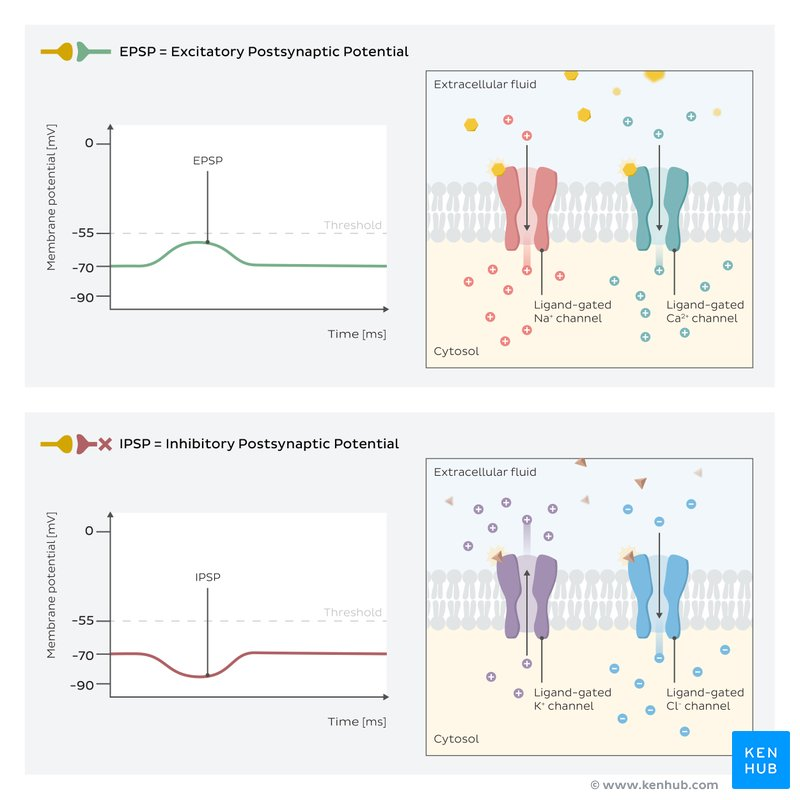
\includegraphics[width=0.65\textwidth]{bilder/ipsp.jpg}
    \quelle{\cite{kenhub_psp}}    
    \caption{Darstellung des Einflusses eines EPSPs und IPSPs auf das Membranpotential}
    \label{IPSP}
\end{figure}




\section{Aufbau und Funktionsweise eines EEG-Systems}
Katharina \newline
\subsection{Grundlegende Messmethode eines EEG-Systems}
Starke Spannungsänderungen auf der Kopfhaut deuten auf eine erhöhte Aktivität des darunterliegenden Gehirns und damit auf kognitive Prozesse hin. Die Elektroenzephalographie hat das Ziel, diese elektrischen Gehirnaktivitäten zu erfassen und aus ihnen Rückschlüsse auf Denkprozesse zu ziehen. Hierzu werden Spannungsdifferenzen mithilfe von Elektroden gemessen.\newline

Eine Elektrode ist ein elektrischer Leiter, der zusammen mit einer Gegenelektrode mit einem Medium, das sich zwischen beiden Elektroden befindet, in Wechselwirkung steht. Sie bestehen meist aus Metall oder Graphit und ermöglichen die Messung von Spannungsunterschieden.\footnote{Vgl. \cite{heinen_elektronik_elektroden}} \newline
Werden zwei Elektroden nah an der Kopfhaut angebracht, erfassen sie die Spannungsdifferenz zwischen den jeweiligen Messorten. Beide Elektroden messen nicht nur die Spannung, die durch Gehirnaktivität entstand, sondern weitere Spannungen, die unabhängig von der Aktivität aufgrund elektrischer Geräte in der Umgebung erzeugt wird. Wird eine Elektrode an einem Ort angebracht, an dem keine Hirnaktivität zu messen ist, ist die Spannungsdifferenz gleich der allein durch Gehirnaktivität an der anderen Elektrode erzeugten Spannung.
Auf diese Weise lässt sich die Gehirnaktivität in der Umgebung einer Elektrode über längere Zeiträume hinweg aufzeichnen. Durch den Einsatz mehrerer Elektroden können Signale aus unterschiedlichen Hirnregionen gleichzeitig erfasst werden, wobei sich die gemessenen Muster je nach Funktion der jeweiligen Region unterscheiden. Diese Methode wird als EEG bezeichnet. Die Aufzeichnungen lassen sich durch Weiterverarbeitung in interpretierbare Muster übersetzen. Mit diesen Informationen können Rhythmen bestimmt und bestimmte Aktivitäten provoziert werden. \newline
Eine Einschränkung bei der EEG ist die räumliche Auflösung. Die elektrischen Signale entstehen in Nervenzellen, über einen Zentimeter von der Kopfhaut entfernt, während die Messung an der Kopfhaut erfolgt. Zwischen diesen Orten befindet sich ein räumlicher Unterschied, auf dem sich die Signale verbreiten. Außerdem erzeugen nur große Flächen gleichzeitig aktiver Neuronen messbare Signale. Die Elektroden messen demnach nicht nur die Spannung eines einzelnen Punktes, sondern einer Fläche von mindestens $6$ $cm^2$.\footnote{Vgl. \cite{stlouis2016}, Appendix 1} Dieser Umstand hat zur Folge, dass empfnagene Signale nicht örtlich einzuordnen sind und keine leichten Rückschlüsse auf den Ort des Signals geschlossen werden können. Das macht EEG zu einer unpraktischen Methode für die örtliche Auflösung von Hinrsignalen. Im Gegensatz dazu ist jedoch die zeitliche Einordnung sehr exakt. Das bedeutet, dass zwischen dem Zeitpunkt, an dem Neuronengruppen aktiviert werden, und dem, an dem das elektrische Signal die Elektroden erreicht und aufgezeichnet wird, nahezu keine Zeit (ungefähr 1 ms)\footnote{Vgl. \cite{tu_darmstadt2022}} vergeht. 

\subsection{Geschichte und aktueller Stand der Forschung}
Richard Caton hat als Erster Messungen von Gehirnaktivität durchgeführt. Er zeigte in Liverpool, dass Gehirne, in seinen Messungen von Affen und Kaninchen, elektrische Ströme erzeugen, die durch Sinnesreize beeinflusst werden. Als \qt{Entdecker der Elektroenzephalographie} gilt jedoch ein Neurologe aus Jena. Hans Berger führte 1924 die ersten Elektroenzephalographien (EEGs) an der Universität Jena durch. Er entdeckte auch den Berger-Effekt, eine auffällige Veränderung des EEGs, die auffällig und damit leicht messbar ist.\footnote{Vgl. \cite{wiki_eeg}}\newline

Seit der Entwicklung des ersten EEG haben zahlreiche Institutionen, Unternehmen und Forschende daran gearbeitet, sowohl die Messgenauigkeit zu verbessern als auch neue Einsatzmöglichkeiten zu erschließen. Dabei lassen sich die Fortschritte und Anwendungen des EEG nach unterschiedlichen Anwendungsbereichen strukturieren.\newline
 Ein zentraler Fokus liegt auf der Verbesserung der Messqualität, da genauere Daten die Grundlage für alle weiteren Anwendungen bilden. Durch Anpassungen an verschiedenen Komponenten des EEG-Geräts können Abweichungen von der tatsächlichen Gehirnaktivität reduziert werden. Ein besonders fortschrittliches System (Stand 2023) stammt von Neuroscan und wird häufig in der Industrie eingesetzt, da es sowohl in Hard- als auch Software vielen anderen EEG-Geräten überlegen ist. Auch Brain Products, ein deutsches Unternehmen, hat zur Weiterentwicklung beigetragen, etwa durch die Entwicklung eines EEG-Headsets mit 160 Elektroden. Dieses ist deutlich dichter als herkömmliche Systeme, die meist maximal 128 Elektroden verwenden.\newline
 Ein wichtiger Anwendungsbereich sind sogenannte \Glspl{brain-computer-interface}. Hierbei wird die Gehirnaktivität erfasst, analysiert und in Steuersignale umgewandelt. Systeme wie das von NeuSen W wurden gezielt für diesen Zweck entwickelt. BCI stellen somit eine konkrete Anwendung der Neurotechnik dar.
 EEG-basierte BCI-Technologien finden besonders im medizinischen Bereich Verwendung. Dazu zählen unter anderem Rehabilitation, Epilepsie-Diagnostik, Emotionserkennung und neurodegenerative Erkrankungen wie Alzheimer und Parkinson.\footnote{Vgl. \cite{wiki_neurodegenerativ}} Durch die Auswertung von Gehirnaktivität eröffnen sich vielfältige Möglichkeiten: So könnten gelähmte Körperteile wieder nutzbar gemacht, Texte ohne Muskelbewegung geschrieben oder Schlafstörungen erkannt werden.\footnote{Vgl. \cite{liu2025}, S. 14} \newline
Im militärischen Bereich werden EEGs eingesetzt, beispielsweise zur Beurteilung von Schädel-Hirn-Traumata infolge von Unfällen.\footnote{Vgl. \cite{fanter1986}} \newline
 Einige Anwendungen befinden sich noch in der Entwicklung, da sie eine noch höhere Messgenauigkeit erfordern. Dennoch gibt es bereits heute realisierbare Ansätze. Ein Forschungsteam der Tsinghua-Universität entwickelte ein BCI mit einer Genauigkeit von etwa 80 \%, mit dem ein Roboterarm gesteuert werden konnte.\footnote{Vgl. \cite{qin2023}, S. 3} Durch gezielte Veränderung des eigenen Gemütszustands gelang es, Hindernisse zu umgehen und Objekte zu greifen.

\subsection{Einteilung der Geräte}
Um einen Vergleich zwischen EEG-Geräten zu ermöglichen, werden sie grundsätzlich in drei Kriterien unterschieden, den Elektroden, der Art der Übertragung zur Weiterverarbeitung und dem Anwendungsbereich. \newline
Die Elektroden können sich auf der Kopfhaut befinden, dann sind sie nicht-invasiv. Die Alternative sind invasive Elektroden, wobei sie beispielsweise ins Gewebe (tiefe Elektroenzephalographie) oder direkt auf den Cortex implantiert werden und sich innerhalb des Schädels befinden. \newline
Anstatt einer herkömmlichen Elektrodenplatzierung und Kabeln als Verbindung nutzen drahtlose Geräte Bluetooth oder andere digitale Übertragungswege, um höhere Flexibilität, Bequemlichkeit und alternative Platzierung der Elektroden zu ermöglichen. Drahtlose Geräte können bei invasiven und nicht-invasiven EEGs eingesetzt werden. \newline
Das letzte Kriterium zur Einordnung von Geräten, mit denen EEGs durchgeführt werden, ist der Anwendungsbereich. Die größten Bereiche sind Forschung und Kliniken. Die Geräte, die zur Forschung genutzt werden, besitzen mehr Elektroden und das Ziel ist eine hohe Präzision, um neue Erkenntnisse zu gewinnen. In Kliniken werden EEGs nach klinischen Standards durchgeführt und für medizinische Diagnosen und Überwachungen, auch über lange Zeiträume, genutzt. Dabei ist die Bequemlichkeit wichtiger als in der Forschung.\footnote{Vgl. \cite{qin2023}, S. 1 und 2}

\subsection{Allgemeiner Aufbau der Geräte}
EEG-Geräte bestehen aus vier grundlegenden Komponenten: Elektroden, Vorverarbeitungsschaltungen, \acrshort{adc}s (kur für \Gls{analog-digital-converter}) und Signalsteuerung und -feedback.\footnote{ Vgl. \cite{qin2023}, S. 4}
Elektroden werden in drei Kategorien unterteilt: invasiv, nicht-invasiv-nass und nicht-invasiv-trocken.\newline
Die Nutzung von nicht-invasiven Elektroden ist ein sicherer und chirurgiefreier Ansatz. Beispiele für solche Elektroden sind Mikronadeln (Abbildung \ref{Spitze Elektroden}), die leicht in die Haut einstechen und so den Neutronen näher sind, und fingerförmige Elektroden (Abbildung \ref{Fingerelektroden}), die leicht durchs Haar dringen und angenehmer sind als Mikronadeln. Beide üben keinen Druck auf den Kopf aus und liegen direkt am Kopf an, was die Stabilität und Genauigkeit erhöht. Die elektrischen Signale sind jedoch gestreut und geschwächt, bevor sie gemessen werden, was die Qualität der aufgenommenen Daten verringert.\footnote{ Vgl. \cite{qin2023}, S. 4 und 5}\newline
Trockene Elektroden bestehen aus einem leitfähigen Material wie Metall und liegen eng am Kopf an. Bei nassen Elektroden wird ein flüssiger \Gls{elektrolyt} verwendet, wie eine Salzlösung oder ein leitfähiges Gel. Das Elektrolyt sorgt für eine bessere elektrische Verbindung zwischen den Elektroden und der Kopfhaut, also weniger Widerstand, kann jedoch austrocknen und ist deswegen nicht für langfristige Nutzung geeignet.\footnote{ Vgl. \cite{anchuang_elektrodenkappe}} \newline

\begin{comment}
\begin{minipage}{0.5\textwidth}
	\includegraphics[width=\textwidth]{bilder/finger_electrodes.jpg}
    \quelle{\cite{xing2018}}
	\captionof{figure}{Fingerelektroden}
    \label{Fingerelektroden}
\end{minipage}
\begin{minipage}{0.5\textwidth}
	\includegraphics[width=\textwidth]{bilder/spikey_electrodes.jpg}
    \quelle{\cite{openbci_ultracortex_shop}}
    \captionof{figure}{Spitze Elektroden}
    \label{Spitze Elektroden}
\end{minipage}
\end{figure}
\end{comment}

\newsavebox{\imgbox}% To store stuff

\begin{figure}[H]
  \centering
  \begin{minipage}[b]{.45\linewidth}
    \centering
    \global\setbox\imgbox=\hbox{\includegraphics[width=\linewidth]{bilder/finger_electrodes.jpg}}% Save largest image
    \usebox\imgbox% Print image
    \par\vspace{0.1cm}\noindent Quelle: \cite{xing2018}\par
    \caption{Fingerelektroden}
    \label{Fingerelektroden}
  \end{minipage}
  \hfill
  \begin{minipage}[b]{.45\linewidth}
    \centering
    \raisebox{\dimexpr0.5\ht\imgbox-0.5\height}{\includegraphics[width=\linewidth]{bilder/spikey_electrodes.jpg}}
    \par\vspace{0.1cm}\noindent Quelle: \cite{openbci_ultracortex_shop}\par
    \caption{Spitze Elektroden}
    \label{Spitze Elektroden}
  \end{minipage}
\end{figure}


Der Nachteil der Schwächung ist bei der Nutzung invasiver Elektroden (Abbildung \ref{invasiv}) nicht oder weniger vorhanden. Die raumzeitliche Auflösung ist höher, je näher die Elektroden den Neuronen, also den Quellen der Signale sind. Das ermöglicht ein tieferes Verständnis von Gehirnregionen und neuronalen Schaltkreisen. 
Die Nachteile sind das Risiko der chirurgischen Implantation, die fortgeschrittene und spezialisierte Herstellung, professionelle Operationen, die für die Messung durchgeführt werden müssen, höhere Kosten, sowie dass ethische Gründe den Einsatz oft verhindern.\footnote{ Vgl. \cite{qin2023}, S. 6}

\begin{figure}[H]
	\centering
	\includegraphics[width=0.5\textwidth]{bilder/invasive_electrode.jpg}
    \quelle{\cite{lee2022}}
    \captionof{figure}{Beispiel für invasive Elektroden}
    \label{invasiv}
\end{figure}

Bei der Verwendung nicht-invasiver Elektroden gibt es verschieden Möglichkeiten, diese anzuordnen. Die Formation ist anhängig von der Anzahl der Elektroden und der fokussierten Hirnrgeionen. Die besonders für nicht-invasive ELektroden standardisierte Elektrodenplatzierung ist das 10-20-System für 21 Elektroden, welches seit 1958 der Standard für klinische Messungen ist. Dabei sind die Messpunkte gleichmäßig verteilt. Viele Systeme arbeiten mit Kappen, an denen die Elektroden feste Plätze haben und nach dem 10-20-System angebracht werden. 10 und 20 stehen dabei für Prozentsätze, die den Winkel zwischen den Elektroden bestimmen (Abbildung \ref{1020sys}). Weiterentwicklungen dieses Systems, wenn mehr Elektroden genutzt werden, werden 10-10-System und 10-5-System genannt.\footnote{ Vgl. \cite{doccheck_1020-system}}

\begin{figure}[H]
	\centering
	\includegraphics[width=0.75\textwidth]{bilder/1020_system.jpg}
    \quelle{\cite{doccheck_1020-system}}
    \caption{Die Anorndung der Elektrodnen nach 10-20-System von der Seite und von oben betrachtet}
    \label{1020sys}
\end{figure}

Jede Elektrode wird mit einem Buchstaben und einer Ziffer kodiert (in manchen Fällen mit zwei Buchstaben). Die Buchstaben sind Abkürzungen für die darunterliegenden Lappen des Gehirns. Sie orientieren sich an den Gehörgangsöffnungen und an zwei festen Punkten, dem Nasion und Inion. Der Punkt Nasion ist in Abbildung \ref{nasion} markiert und der am weitesten vorne gelegene Punkt der Nahtstelle zwischen Stirnbein und linken und rechten Nasenbein. Die horizontale Ebene, auf der dieser Punkt liegt, trennt das Ober- vom Mittelgesicht.\footnote{Vgl. \cite{doccheck_nasion}} Der Punkt, der mit Inion bezeichnet wird, ist der am weitesten vorspringende Punkt des Os occipitalem, ein platter Schädelknochens an der hinteren unteren Seite des Schädels und in Abbildung \ref{inion} markiert.\footnote{Vgl. \cite{doccheck_inion}} \newline

\begin{minipage}{0.5\textwidth}
	\includegraphics[width=\textwidth]{bilder/nasion.jpg}
    \quelle{\cite{doccheck_nasion}}
	\captionof{figure}{Position des Nasions}
    \label{nasion}
\end{minipage}
\begin{minipage}{0.5\textwidth}
	\includegraphics[width=\textwidth]{bilder/inion.jpg}
    \quelle{\cite{doccheck_inion}}
	\captionof{figure}{Position des Inions}
    \label{inion}
\end{minipage}

Die Buchstaben stehen für:
\begin{itemize}

    \item Fp = präfrontal - über präfrontalen Cortex
    \item F = frontal - über Frontallappen
    \item C = central - auf Verbindungslinie zwischen Gehörgangsöffnung, in der Mitte der sagittalen (Nasion zu Inion) Linie
    \item T = temporal - über Temporallappen
    \item P = parietal - über Parietallappen
    \item O = okzipital - über Okzipitallappen
    \item A = aurikulär - am Ohr
    \item Z = zero (null) - ersetzt die Zahl an Elektroden zwischen Nasion und Inion, in der Mitte der koronaren (linke zu rechte Gehörgangsöffnung) Linie\footnote{Vgl. \cite{doccheck_1020-system}}

\end{itemize}
Elektroden, die auf der rechten Seite des Kopfes (rechts der sagittalen Linie) anliegen, werden mit einer geraden Nummer kodiert, links liegende mit einer ungeraden Nummer. Alle Zahlen nehmen von Nasion zu Inion und von zentral zu temporal zu.\footnote{Vgl. Ebd.}
    

Mit Z bezeichnete Elektroden werden oft als Referenzelektroden genutzt, da sie keiner Gehirnhälfte angehören und aufgrund ihrer Position keine Neuronenaktivität aufzeichnen.
Referenzelektroden spielen bei der Messung und im nächsten Schritt eine Rolle: der Vorverarbeitung. Diese geschieht durch Filter, Verstärker und die Ground- und Referenzelektroden.
Die Filter eliminieren ungewollte Störungen, behalten jedoch die Hauptfrequenz bei. Verstärker werden eingesetzt, um die geringen Amplituden des Signals (das Rohsignal liegt im Mikrovoltbereich) zu erhöhen (zum Beispiel in den Millivoltbereich), dadurch wird es einfacher, sie digital aufzuzeichnen.\footnote{ Vgl. \cite{qin2023}, S. 8} Referenzelektroden sind an Stellen des Kopfes angebracht, an denen keine Gehirnaktivität zu messen ist und machen einen Spannungsvergleich mit den anderen Elektroden möglich. Die Groundelektrode an Stirn oder Wange misst nur sehr wenig Hirnaktivität, sondern schafft ein gemeinsames elektrisches Bezugspotential für das Messsystem. Wenn sich elektromagnetische Felder in der Umgebung befinden, sich beispielsweise wenn ein Monitor neben der Messanordnung steht, misst die Groundelektrode die dadurch entstandene Spannung. Durch beide Elektroden, Referenz und Ground, ermöglichen Berechnungen in der Vorverarbeitungsschaltung und die weitergegebenen Daten zeigen einzig die Aktivität des Gehirns.\footnote{ Vgl. \cite{biopac_reference_ground}}\newline

Anschließend werden analoge Spannungssignale in digitale Form umgewandelt. Dies geschieht im ADC. Die Daten werden an Prozessoren gesendet, die Echtzeit-Verarbeitung und Analyse von Rohdaten ermöglichen. Sie erstellen die Grundlage für nachfolgende Datenverarbeitung am Computer.
Dort werden die Signale nach Mustern durchsucht. Aus den erkannten und klassifizierten Mustern werden Schlüsse gezogen und, je nach Versuchsaufbau und Anwendungsbereich, Feedback gegeben.\footnote{ Vgl. \cite{qin2023}, S. 7}





\section{Auswertung von durch EEGs erzeugten Daten - Frequenzbandanaylse}
Sophie \newline

\subsection{Grundlagen der EEG-Analyse}

Um EEG-Daten zu verstehen und zu interpretieren, können die Signale in zwei sich ergänzende Perspektiven unterteilt werden.\footnote{Vgl. \cite{wikipedia_eeg_nyquist}} 
Es wird erstens in spontane EEG-Rhythmen unterschieden, welche als kontinuierliche Oszillationen in verschiedenen Frequenzbereichen beobachtet werden können, und zweitens ERPs (aus dem Englischen \emph{event-related potentials}, \glqq ereignisbezogene Potentiale\grqq), welche als zeitlich gebundene Spannungsänderungen in Reaktion auf bestimmte Ereignisse oder Stimuli erscheinen.\footnote{Vgl. \cite{wikipedia_eeg_nyquist}} Zusammen erlauben die Frequenzbänder und die zeitbezogenen ERPs die Analyse der EEG-Daten. 
Im folgenden Abschnitt wird auf die wichtigsten Frequenzbänder des EEGs und den Ursprung der ERPs eingegangen. Anschließend werden wichtige Störgrößen wie Rauschen und Artefakte erklärt, um aus EEG-Aufzeichnungen aussagekräftige Informationen abzuleiten. 

EEG-Signale enthalten rhythmische Oszillationen, welche historisch in verschiedene Frequenzbänder unterteilt wurden, die mit griechischen Buchstaben bezeichnet wurden. Diese inkludieren $\delta$-, $\theta$-, $\alpha$-, $\beta$- und $\gamma$-Bänder sowie spezielle Bänder wie $\mu$ und $\sigma$.\footnote{Vgl. \cite{nayak_waveforms}}  Jedes Band wird mit bestimmten Gehirnzuständen oder Funktionen assoziiert. In der Praxis können diese Bänder von den rohen EEG-Daten durch Spektralanalysetechniken (z.B. Fourier-Transformationen oder Welch-Verfahren) extrahiert werden, was oft als quantitative EEG Analyse bezeichnet wird. \footnote{Vgl. \cite{wikipedia_eeg_nyquist}}  

Unter einem Frequenzband wird dabei ein definierter Frequenzbereich verstanden, in dem charakteristische EEG-Aktivität auftritt. Die elektrische Aktivität selbst beschreibt die im EEG gemessenen Signale, während regelmäßig auftretende, strukturierte Muster dieser Aktivität als Rhythmen bezeichnet werden.

\subsection{Frequenzbänder}

\begin{description}

\item[\textbf{\emph{Delta} ($\boldsymbol{\delta}$)}] 

\textbf{bis zu \textasciitilde 4 Hz}

Delta-Aktivität ist die langsamste Aktivität und weist die höchste Amplitude auf. Sie tritt besonders während des Tiefschlafs und im EEG von Säuglingen auf.\footnote{Vgl. \cite{jadeja2021}} Bei wachen Erwachsenen ist eine diffuse Delta-Aktivität abnormal und kann auf eine Funktionsstörung des Gehirns hinweisen. Delta-Rhythmen treten bei Erwachsenen tendenziell frontal (nach vorne gerichtet) auf (frontale intermittierende rhythmische Delta-Wellen) und bei Kindern posterior (hinten liegend).\footnote{Vgl. Ebd.}

\item[\textbf{\emph{Theta} ($\boldsymbol{\theta}$)}] 

\textbf{\textasciitilde 4-7 Hz}

Theta-Aktivität ist bei Kindern und in schläfrigen oder meditativen Zuständen bei Erwachsenen normal.\footnote{Vgl. \cite{wiki_eeg}} Beispielsweise ist der Übergang zum Schlaf oder die Schläfrigkeit durch eine Zunahme von Theta-Aktivität gekennzeichnet. Übermäßige Theta-Aktivität bei einem wachen Erwachsenen, insbesondere im Lobus frontalis ist abnormal und kann z.B. bei Enzephalopathien (Funktionsstörung des Gehirns, die das Gehirn als Ganzes betrifft) auftreten.\footnote{Vgl. \cite{jadeja2021}}

\item[\textbf{\emph{Alpha} ($\boldsymbol{\alpha}$)}] 

\textbf{\textasciitilde 8-13 Hz}

Der Alpha-Rhythmus war die erste, von Hans Berger entdeckte, beschriebene EEG-Oszillation. Klassischerweise wird sie als ausgeprägter posterior dominanter Rhythmus beobachtet, wenn eine Person wach, aber entspannt ist und beispielsweise ihre Augen schließt.\footnote{Vgl. Ebd.} Alpha-Aktivität hat typischerweise ihre maximale Amplitude über dem Okzipitallappen und wird durch das Öffnen der Augen oder mentale Anstrengung abgeschwächt, ein Phänomen, welches als \glqq Berger Effekt \grqq{} bezeichnet wird.\footnote{Vgl. \cite{jensen2010}} Im Wesentlichen zeigt der Alpha-Rhythmus einen ruhigen, erholsamen Zustand an, welcher verschwindet, wenn wir wachsam werden oder uns aktiv mit Gedanken beschäftigen. Neben dem posterioren Alpha, gibt es andere Varianten, wie z.B. der Mu-Rhythmus über dem sensomotorischen Kortex, welcher mit motorischer Inaktivität assoziiert wird.\footnote{Vgl. Ebd.} Der Mu-Rhythmus wird während Bewegungen oder sogar der reinen Beobachtung von Bewegungen (in Verbindung mit der Aktivität von Spiegelneuronen) unterdrückt (Desynchronisation).\footnote{Vgl. \cite{jadeja2021}} Die Mu-Supression wird häufig in BCI-Anwendungen zur Erkennung motorischer Vorstellungen oder Absichten genutzt. 

\item[\textbf{\emph{Beta} ($\boldsymbol{\beta}$)}] 

\textbf{\textasciitilde 13-30 Hz}

Beta-Aktivität hat höhere Frequenzen, kleinere Amplituden und kommt häufig in frontalen Regionen des Kortexes vor. Sie wird mit Wachsamkeit, aktivem Denken und Konzentration assoziiert.\footnote{Vgl. Ebd.} Die Beta-Aktivität mit niedriger Amplitude steigt bei Aufgaben, die Aufmerksamkeit oder geistige Anstrengung erfordern, und ist der dominante Rhythmus bei geöffneten Augen oder wenn der Geist aktiv ist.\footnote{Vgl. Ebd.} Beta-Aktivität steht auch mit motorischem Verhalten in Verbindung, sie ist während der motorischen Vorbereitung vorhanden und wird typischerweise während der eigentlichen Bewegung unterdrückt (ein Beispiel für ereignisbezogene Desynchronisation).\footnote{Vgl. \cite{wiki_eeg}} Nach der Bewegung kann es zu einem Rebound der Beta-Leistung kommen, einem vorübergehenden Wiederanstieg der Beta-Aktivität nach ihrer Unterdrückung, welcher darauf zurückgeführt wird, dass sich neuronale Netzwerke nach der Bewegung wieder synchronisieren und ihre charakteristische Aktivitätsdynamik erneut ausbilden, einem Phänomen, welches in der motorischen EEG Analyse von Relevanz ist. Im klinischen Kontext kann eine verstärkte rhythmische Beta-Aktivität bei bestimmten Sedativa (z.B. Benzodiazepinen)\footnote{Vgl. \cite{vanlier2004}} oder Pathologien (z.B. im EEG von Patienten mit Dup15q-Syndrom) beobachtet werden. Im Gegensatz dazu kann ein Verlust der Beta-Aktivität in einer Region auf eine Schädigung der Großhirnrinde hindeuten.\footnote{Vgl. \cite{wiki_eeg}}

\item[\textbf{\emph{Gamma} ($\boldsymbol{\gamma}$)}] 

\textbf{ab \textasciitilde 30 Hz (bis zu \textasciitilde 100 Hz)}

Gamma ist das Frequenzband mit der höchsten Frequenz, welches üblicherweise im EEG analysiert wird. Gamma-Aktivität weist eine relativ geringe Amplitude auf und wird mit hochgradigen kognitiven Prozessen in Verbindung gebracht. Eine Theorie besagt, dass die Gamma-Aktivität die Verbindung verteilter neuronaler Populationen zu kohärenten Netzwerken für kognitive oder motorische Funktionen widerspiegelt, indem sie mit einer zeitlichen Synchronisation der Aktivität dieser räumlich getrennten Neuronen einhergeht, sodass Informationen effizient integriert und verarbeitet werden können.\footnote{Vgl. Ebd.} Beispielsweise können vorübergehende Steigerungen der Gamma-Aktivität mit Aufmerksamkeit oder multisensorischer Integration (Verbindung von Informationen verschiedener Sinnesorgane) korrelieren. Die zuverlässige Erkennung von Gamma-Aktivität auf der Kopfhaut kann jedoch schwierig sein, da Muskelartefakte (z.B. Anspannen der Kiefermuskeln) ebenfalls hochfrequente Signale erzeugen, die das EEG im Gamma-Bereich verfälschen können.\footnote{Vgl. \cite{jia2011}}  Dies kann jedoch durch geeignete Filterung reduziert werden. 

\end{description}

\subsection{Weitere Rhythmen}

Zusätzlich zu diesen Bändern existieren weitere benannte Rhythmen, wie der oben benannte Mu-Rhythmus. Ein weiterer ist das Sigma-Band (12-16 Hz), welches sich als sogenannte Schlafspindel zeigt und eher kurze Sprunghafte Aktivitäten kennzeichnet.\footnote{Vgl. \cite{uchida1991}}

\subsection{Mit Frequenzbändern assoziierte Zustände}
\begin{table}[h]
\centering
\caption{Übersicht der EEG-Frequenzbänder und ihrer typischen Zustände}
\begin{tabular}{lll}
\textbf{Frequenzband} & \textbf{Frequenzbereich} & \textbf{Typischer Zustand} \\
\hline
Delta ($\boldsymbol{\delta}$) & bis \textasciitilde 4 Hz & Tiefschlaf \\
Theta ($\boldsymbol{\theta}$) & \textasciitilde 4--7 Hz & Schläfrigkeit, Meditation \\
Alpha ($\boldsymbol{\alpha}$) & \textasciitilde 8--13 Hz & Entspannung, Wachzustand \\
Beta ($\boldsymbol{\beta}$) & \textasciitilde 13--30 Hz & Konzentration, Aktivität \\
Gamma ($\boldsymbol{\gamma}$) & ab \textasciitilde 30 Hz & kognitive Verarbeitung \\
\end{tabular}
\end{table}

\subsection{Bedeutung und Anwendungen}

 Die Frequenzbandanalyse ist auch für viele Anwendungen von besonderer Bedeutung. Im klinischen Kontext werden EEG-Rhythmen genutzt, um Anomalien zu identifizieren und BCI-Forscher entwickeln Systeme zur gezielten Modulation bestimmter Bänder. Eine klassische Applikation ist das Nutzen der Alpha- oder Beta-Rhythmusmodulation für die BCI-Steuerung, wie Beispielsweise, wenn eine Person lernt, ihre Alpha-Leistung zu Steigern, um einen Befehl auszuführen oder die Mu-/Beta-Suppression um eine Prothese zu steuern. Studien zeigten, dass eine einfache binäre Kontrolle durch die Erkennung von Veränderungen im EEG erreicht werden kann. In einer frühen Demonstration erlernte ein gelähmter Patient Beta Aktivität zu nutzen, um einen Schalter zu bedienen, welcher einen Computer Cursor bewegte und zusätzlich elektrische Stimulatoren für seine Hand aktivierte. Dadurch konnte der Patient ein gewisses Maß an Bewegungsfreiheit zurückgewinnen.\footnote{Vgl. Ebd.}

\subsection{Event-Related Potentials}

Während EEG-Rhythmen den generellen Zustand des Gehirns widerspiegeln, sind Event-Related-Potentials neuronale Reaktionen, welche mit bestimmten sensorischen, kognitiven oder motorischen Ereignissen verbunden sind und aus dem gesamten EEG extrahiert werden können.\footnote{Vgl. \cite{luck2005}, S. 4} Da jede ereignisausgelöste neuronale Reaktion sich  klein im Vergleich zu EEG-Schwankungen verhält, werden in den meisten EEG-Experimenten ERP-Wellen durch verschiedene Signalmittelungen von zufälligen Hintergundrauschen isoliert.\footnote{Vgl. \cite{luck2005}, S. 56}

\subsection{ERP-Komponenten}

ERP-Komponenten bestehen aus einer Serie von positiven und negativen Spannungsdeflexionen und werden anhand ihrer Polarität (P für positive oder N für negative Spannung relativ zur Basislinie (normale elektrische Gehirnaktivität eines Menschen im Ruhezustand)) sowie ihres typischen Zeitverlaufs gekennzeichnet.

\subsubsection{Zeitlicher Ablauf der ERP-Komponenten}

\textbf{C1-} Die erste wichtige ERP-Komponente wird als C1 bezeichnet und ist an den hinteren Mittelinienelektrodenstellen am größten. Im Gegensatz zu anderen Komponenten ist sie nicht mit P oder N gekennzeichnet, da ihre Polarität variieren kann.\footnote{Vgl. \cite{luck2005}, S. 35} Die an der Kopfhaut gemessene Spannung bei Reizen im unteren Gesichtsfeld ist positiv und bei Reizen im oberen Gesichtsfeld negativ. Die C1-Komponente entsteht im V1 (primärer visueller Kortex) und tritt typischerweise etwa 40-60 ms nach dem Reiz auf und erreicht ihren Höhepunkt 80-100 ms nach dem Reiz. Sie ist sehr anfällig für Stimulusparameter, wie Kontrast (Helligkeitsunterschiede im Reiz, welche die Stärke der neuronalen Antwort beeinflussen, da stärkere Kontraste zu einer höheren Aktivierung visueller Neuronen führen) und räumliche Frequenz (Feinstruktur bzw. Detailgrad eines visuellen Reizes, da unterschiedliche Frequenzen von verschiedenen Neuronenpopulationen im visuellen Kortex verarbeitet werden).\footnote{Vgl. Ebd.}\newline

\textbf{P1-} Die positive P1-Komponente erreicht an den lateral okzipitalen Elektroden ihre maximale Amplitude und tritt 60-90 ms nach dem Reiz auf und erreicht ihr Maximum bei 100-130 ms. Sie ist allerdings schwierig genau zu identifizieren, da sie sich mit der C1-Welle überlappt. Zusätzlich ist anzumerken, dass die P1-Latenz sich maßgeblich durch den Stimuluskontrast verändern kann.\footnote{Vgl. \cite{luck2005}, S. 36}\newline

\textbf{N1-} Die N1-Welle hat mehrere Subkomponenten. Die früheste Subkomponente erreicht ihr Maximum 100-150 ms nach dem Reiz an anterioren Elektroden. Des Weiteren gibt es mindestens zwei N1-Komponenten, welche posterior 150-200 ms nach dem Reiz ihren Höhepunkt erreichen. Eine davon entsteht im parietalen Kortex und die andere im lateral okzipitalen Kortex.\footnote{Vgl. \cite{luck2005}, S. 37} \newline

\textbf{P2-} Die P2-Welle wird vor allem an anterioren und zentralen Bereichen der Kopfhaut gemessen und tritt typischerweise im Zeitbereich von etwa 150-250 ms nach dem Reiz auf. Sie überlappt sich oft mit N1-und N2-Wellen, wodurch sie schwer isolierbar ist und somit wenig über sie bekannt ist.\footnote{Vgl. Ebd.}


\subsection{Einflussfaktoren und Störgrößen}

Um aufschlussreiche Ergebnisse aus der EEG Analyse zu gewinnen, müssen einige wichtige Aspekte berücksichtigt werden. EEG Signale sind von Natur aus schwach und sehr verrauscht und viele technische und psychologische Faktoren können die Messung beeinflussen. Im Folgenden werden einige Punkte aufgeführt, welche bei EEG-Experimenten beachtet werden müssen.

\textbf{Artefakte und Rauschen:} EEG Aufzeichnungen sind grundsätzlich mit Artefakten kontaminiert. Artefakte sind Signale, welche nicht von der Gehirnaktivität stammen.\footnote{Vgl. \cite{wiki_eeg}} Häufige Artefakte umfassen Augenblinzeln und Augenbewegungen (diese produzieren große Spannungsabweichungen durch das Stehpotential des Auges), Muskelaktivität (Gesichts- und Nackenmuskeln können hochfrequente Störgeräusche verursachen), Herzsignale (der Puls kann rhythmische Störungen verursachen) und externe elektrische Störungen (Netzstromstörungen bei 50/60 Hz) sowie Schweißbildung auf der Kopfhaut (Elektrolyte im Schweiß können die Leitfähigkeit verändern und dadurch langsame Signalverschiebungen oder Drift verursachen).\footnote{Vgl. Ebd.} Da einige Artefakte echte Gehirnströme imitieren oder verdecken können (z.B. können Verspannungen der Kopfhautmuskulatur eine Frequenz von 20-30 Hz erzeugen, welche fälschlicherweise als Beta oder Gamma interpretiert werden könnten), ist ein sorgfältiger Umgang mit Artefakten entscheidend.\footnote{Vgl. Ebd.} Dies kann vorbeugende Maßnahmen (z.B. Hinweise an den Probanden, Bewegungen zu minimieren) sowie Nachbearbeitungsmethoden umfassen. Eine Möglichkeit ist beispielsweise die Filterung (z.B. Verwendung eines \gls{notch} bei 50 Hz, um Netzrauschen zu vermeiden). Doch Filtern allein reicht oft nicht aus, da sich Artefakte mit den für die Analyse relevanten Frequenzbändern überlappen.\footnote{Vgl. \cite{acns_guideline2}} Komplexere Methoden wie \acrshort{ica} (kurz für \gls{icalang}) oder statistische Regression können angewendet werden, um einzelne Artefakte herauszufiltern (z.B. das Isolieren eines Augenblinzelartefakts).\footnote{Vgl. \cite{acns_guideline2}} Bei der Validierung eines EEG-Geräts muss geprüft werden, dass das System eine ausreichende Signalqualität mit wenig Rauschen aufweist, sodass Artefakte zuverlässig entfernt werden können und die zu messenden Gehirnströme nicht in Verstärkerrauschen oder Interferenz untergehen.\footnote{Vgl. \cite{acns_guideline2}} 

\textbf{Elektrodenanordnung und Referenz:} Da EEG-Messungen Spannungsunterschiede messen, hat die Wahl einer Referenzelektrode signifikanten Einfluss auf die aufgezeichneten Wellen. Das liegt daran, dass es keinen neutralen Punkt am Körper gibt (das sogenannte “No Switzerland principle“\footnote{Vgl. \cite{acns_guideline2}}), sodass jede Referenzwahl (egal ob am Ohrläppchen, Mastoid (Teil des Schläfenbeins hinter dem Ohr), Vertex Cz oder einem Durchschnitt aller Elektroden) einen gewissen Bias oder ein Profil auf den Daten hinterlässt. Beispielsweise können, wenn eine frontale Referenzelektrode gewählt wurde, alle Signale relativ zu einer Mastoidreferenz invertiert erscheinen.\footnote{Vgl. \cite{wikipedia_eeg_nyquist}} Viele moderne EEG-Systeme erlauben es, später die Referenz zu ändern (z.B. zur Durchschnittsreferenz). Bei der Validierung eines Geräts muss daher darauf geachtet werden, dass bei beiden Geräten dieselbe Referenz genutzt wird. Ebenfalls ist die standardisierte Elektrodenanordnung (internationales 10-20 System) wichtig, um sicherzustellen, dass bekannte Muster in den korrespondierenden Kanälen angezeigt werden.\footnote{Vgl. \cite{acns_guideline2}} 

\textbf{Filter und Signalbandbreite:} EEG-Signale umfassen ein breites Spektrum an Frequenzen, von langsamen (\acrshort{dc}, kur für \acrlong{dc}) (< 0,5 Hz) bis zu 100 Hz oder mehr.\footnote{Vgl. \cite{wikipedia_eeg_highpass}} Um sich auf die relevanten Frequenzbänder zu fokussieren und Rauschen zu reduzieren, werden normalerweise \gls{bandpass} angewendet, welcher Signale über einer bestimmten \gls{cutoff} passieren lässt. Ein gängiger Bandpass für Aufzeichnungen von EEGs bei Erwachsenen liegt beispielsweise bei ca. 0,1 Hz (Hochpassfilter) bis 100 Hz (Tiefpass), wodurch der herkömmliche Delta- bis Gammabereich erhalten bleibt und hochfrequente Störgeräusche sowie langsame Verschiebungen herausgefiltert werden.\footnote{Vgl. \cite{wikipedia_eeg_highpass}} Es ist von essentieller Bedeutung, vor der Analyse geeignete Filtereinstellungen zu wählen. So kann beispielsweise ein zu hoher Hochpassfilter langsame Wellen und ERPs verzerren, während ein zu niedriger Tiefpassfilter Komponenten wie Spikes oder Hoch-Beta-Oszillationen dämpfen kann.\footnote{Vgl. \cite{acns_guideline2}} Tatsächlich haben Forscher herausgefunden, dass die Verwendung einer Hochpassgrenzfrequenz von 0,5 Hz gegenüber 0,01 Hz die scheinbare Amplitude der \gls{p300} erheblich reduzieren kann, was unterstreicht, wie sich die Wahl des Filters auf die gemessenen Signale auswirkt.\footnote{Vgl. \cite{acns_guideline2}}   

\textbf{Subjektfaktoren und Versuchsaufbau:} EEG-Systeme reagieren sehr empfindlich auf den Zustand des Probanden und den Versuchsaufbau. Vor der Analyse der Daten müssen Faktoren wie der Wachheitsgrad, die Müdigkeit und die Bewegungen des Probanden sowie Faktoren wie Raumgeräusche oder Änderungen der Elektrodenimpedanz betrachtet werden. Viele dieser Faktoren können die Ergebnisse beeinflussen oder verfälschen: So weist beispielsweise ein schläfriger Proband mehr Theta-Wellen auf und kann somit die Basislinie der \qt{Alpha-/Betaleistung} verzerren.\footnote{Vgl. \cite{nayak_waveforms}} Ein weiteres Beispiel ist, wenn die Probanden sich während der Aufzeichnung langweilen, wodurch überdurchschnittlich viel Alpha produziert wird. Daher ist es wichtig, den Zustand des Probanden zu kontrollieren oder zu überwachen (manche Protokolle quantifizieren sogar Augenblinzeln oder inkludieren \acrshort{eog}-Kanäle (kurz für \gls{elektrookulogramm}), um die Wachsamkeit zu berücksichtigen).\footnote{Vgl. \cite{nayak_waveforms}} Für ERPs muss das experimentelle Paradigma gut designt sein. Stimuli sollten mit präzisem Timing präsentiert werden (oft unter Verwendung von \gls{eventmarker}) und der Versuch mit hinreichender Wiederholung durchgeführt werden, um eine Durchschnittsbildung zu ermöglichen. Sollte ein System auf die Fähigkeit, eine \gls{p300}-Welle zu erfassen, validiert werden, würde eine \gls{oddball} mit klar definierten Ziel- und Standardreizen entworfen und sichergestellt werden, dass der Teilnehmer engagiert ist, damit ein robustes P300 ausgelöst wird.\footnote{Vgl. \cite{acns_guideline2}} Die Konsistenz zwischen den Versuchen und Probanden ist entscheidend.

Zusammenfassend zeigt sich, dass die Qualität und Aussagekraft von EEG-Daten maßgeblich von der sorgfältigen Kontrolle technischer, physiologischer und experimenteller Einflussfaktoren abhängt. Nur durch die Berücksichtigung dieser Aspekte können Artefakte minimiert und valide Rückschlüsse auf die zugrunde liegende Gehirnaktivität gezogen werden.

\section{Merkmale von Brain-Computer-Interfaces und mögliche Andwendungen}
Alisa \newline

Die zuvor beschriebene Frequenzbandanalyse ist eine wichtige Grundlage für die Funktionsweise von Brain-Computer-Interfaces.
Dabei werden Gehirnsignale in Frequenzbereiche zerlegt, mit gespeicherten Referenzmustern verglichen und charakteristische Signale erkannt. 
Diese können anschließend als Steuerbefehle für technische Geräte benutzt werden.\newline

Ein Brain-Computer-interface ermöglicht eine direkte Informationsübertragung zwischen einem organischen Gehirn und einem technischen System.
Sie nehmen neuronale Signale auf, analysieren und übersetzen diese in Befehle, ohne das eine Muskelbewegung erforderlich ist. 
Dadurch schaffen BCIs völlig neue und kreative Möglichkeiten, Geräte zu steuern, die unabhängig von körperlicher Bewegung oder Sprache funktionieren.\newline

Die Funktionsweise eines BCI beruht auf der kontinuierlichen Erfassung physiologischer Signale, vor allem der elektrischen Aktivität des Gehirn.
Diese wird mithilfe eines Elektroenzephalogramms (EEG) gemessen.
Die Signale, die aufgezeichnet werden, werden mit vorab festgelegten oder erlernten Mustern verglichen, um charakteristische neuronale Signale festzustellen, die gleichzeitig als Kontrollsignale dienen.\footnote{Vgl. \cite{heuer2015}}
Durch die Analyse dieser Kontrollsignale kann das BCI die Intentionen des Benutzers erkennen und diese sodann in Steuerbefehle umsetzen.
Damit ein BCI zuverlässig funktioniert, müssen die Signale möglichst genau ausgewertet und in Echtzeit verarbeitet werden.
Gleichzeitig können äußere Störsignale sowie Unterschiede zwischen den Nutzern die Signalverarbeitung und Interpretation erschweren.
Dies führt dazu, dass die Interpretation der Signale anfällig für Fehler ist und nicht immer zwischen verschiedenen Gehirnaktivitäts- Zuständen unterschieden werden kann.
In der Praxis erfordert dies daher eine ausführliche Signalverarbeitung sowie oft eine Anpassung des Systems an den jeweiligen Nutzer. \newline

Ein vereinfachtes Beispiel wurde für ein BCI System  wurde im Rahmen eines Informatikprojekts in der 10.Klasse umgesetzt.
Dabei wurden EEG-Daten von einem portablen EEG in Echtzeit erfasst, analysiert und als Spiel visuell dargestellt.
Die Auswertung der EEG-Daten basierte auf der Analyse des bestimmten Frequenzbereiches Alpha, die Rückschlüsse auf die mentale Aktivität des Nutzers ermöglichte.
Die Steuerung erfolgte über ein interaktives Spiel, bei welchem ein Ballon abhängig von der Gehirnaktivität gesteuert wurde. Dieses Projekt verdeutlichte die Funktionsweise eines BCI, da auch hier neuronale Signale verarbeitet und in eine visualisierte Auswertung der Gehirnströme überführt wurden.
Während in diesem Projekt nur eine visuelle Rückmeldung erzeugt wurde, lässt sich die gleiche Funktionsweise auf andere reale Systeme übertragen.
So können die analysierten Gehirnsignale auch genutzt werden, um einen Roboterarm, genannt \glqq Arduino Tinker Kit Braccio\grqq{} zu steuern.

\begin{figure}[H]
\centering
   	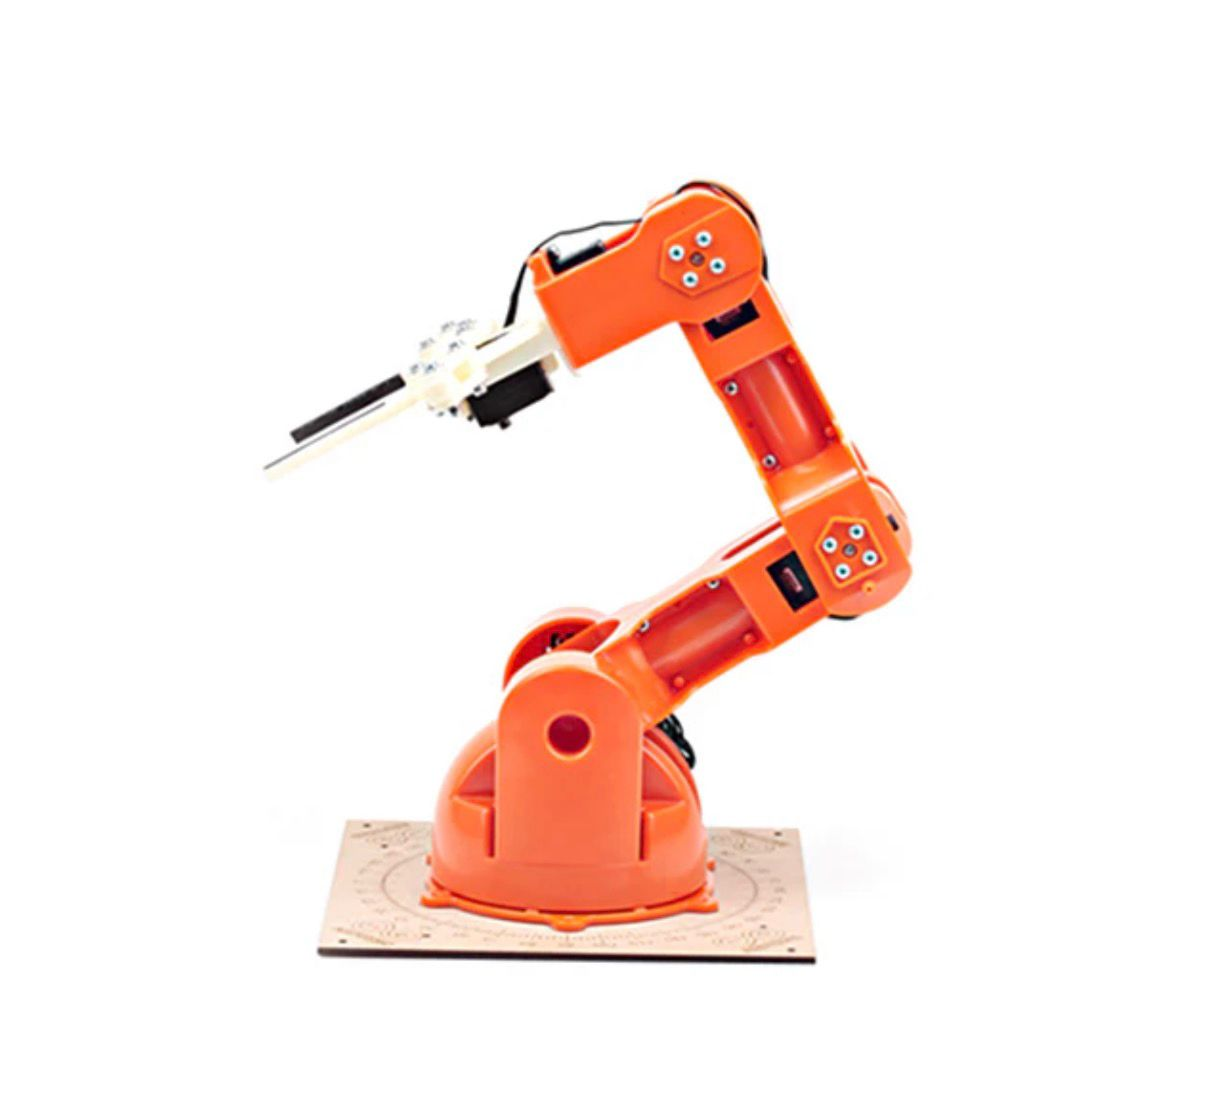
\includegraphics[width=0.5\textwidth]{bilder/roboter.jpeg}
    \quelle{\cite{lee2022}}
    \captionof{figure}{Roboterarm Arduino Tinkerkit Braccio}
    \label{roboter}
\end{figure}


Dabei werden die erkannten Muster nicht mehr nur abgebildet, sondern direkt in physische Bewegungen umgesetzt.
Im Rahmen der Seminarfacharbeit, wird neben der Validierungsstudie eines portablen sowie stationären EEG-Systems zusätzlich die Möglichkeiten zur Steuerung eines Roboterarms mithilfe eines BCI-Programms untersucht und praktisch umgesetzt. \newline

Brain-Computer-Interfaces gewinnen in der heutigen Zeit an Bedeutung.
Insbesondere Menschen mit körperlichen Behinderungen können von der Technik mit der Umsetzung von BCIs profitieren.
Es gibt bereits prototypische Systeme, wie beispielsweise die Steuerung eines Cursors, die Nutzung von Buchstabierprogrammen oder die Kontrolle von prothetischen Geräten ermöglichen.
Neben medizinischen Anwendungen,  gewinnen in den vergangenen Jahren auch nicht-medizinische Einsatzmöglichkeiten an Aufmerksamkeit.
Dazu zählen unter anderem die Steuerung von Fahrzeugen oder Robotern sowie die Überwachung von mentalen Zuständen.


\section{Fragestellung und Hypothesen}



\chapter{Methodisches Vorgehen einer EEG-Validierungsstudie}
\section{Beschreibung der Stichprobe}
\section{Experimentalaufbau für die Messung}
\section{Beschreibung der Messapparatur}




\section{Auswertungsmethodik}

\input{kapitel/Experiment}

\input{kapitel/Ergebnisse}

\input{kapitel/Diskussion}

\addcontentsline{toc}{chapter}{Glossar}

\printglossary


\input{kapitel/Anhang.tex}

\printbibliography[nottype=misc, heading=bibliography, title={Literaturverzeichnis}]

\printbibliography[type=misc, heading=bibliography, title={Internetquellen}]

\listoffigures %Abbildungsverzeichnis

\begin{comment}%Verwendung siehe Präamble
\bibliography{literatur}
\bibliographystyle{dinat}

\bibliographyonline{literatur}
\bibliographystyleonline{dinat}
\end{comment}

\begin{comment}
	

\chapter*{Danksagung}
%Kann auch als Kapitel angelegt werden.

\chapter*{Eidesstattliche Erklärung}
Wir erklären, dass wir die vorliegende Arbeit mit dem Titel \qt{Titel} selbstständig, ohne unzulässige fremde Hilfe angefertigt und nur unter Verwendung der angegebenen Literatur und Hilfsmittel verfasst haben. 
Sämtliche Stellen, die wörtlich oder inhaltlich anderen Werken entnommen sind, wurden unter Angabe der Quellen als Entlehnung kenntlich gemacht. 
Dies trifft besonders auch auf Quellen aus dem Internet zu. Gleichzeitig geben wir das Einverständnis, unsere Arbeit mittels einer Plagiatssoftware durch die Schule überprüfen zu lassen.

\vspace{0.3cm}
\noindent
Ort, den tt. Monat jjjj

\vfill

\noindent\begin{tabular}{ll}
\makebox[2.5in]{\hrulefill} & \makebox[2.5in]{\hrulefill}\\
Vorname Name& Vorname Name\\[8ex]
\makebox[2.5in]{\hrulefill} & \makebox[2.5in]{\hrulefill}\\
Vorname Name & Vorname Name\\
\end{tabular}
%Bei Drei Personen die Felder für Person Vier mit Leerzeichen ersetzen.
\end{comment}

\end{document}
